\documentclass[]{article}
\usepackage{lmodern}
\usepackage{amssymb,amsmath}
\usepackage{ifxetex,ifluatex}
\usepackage{fixltx2e} % provides \textsubscript
\ifnum 0\ifxetex 1\fi\ifluatex 1\fi=0 % if pdftex
  \usepackage[T1]{fontenc}
  \usepackage[utf8]{inputenc}
\else % if luatex or xelatex
  \ifxetex
    \usepackage{mathspec}
  \else
    \usepackage{fontspec}
  \fi
  \defaultfontfeatures{Ligatures=TeX,Scale=MatchLowercase}
\fi
% use upquote if available, for straight quotes in verbatim environments
\IfFileExists{upquote.sty}{\usepackage{upquote}}{}
% use microtype if available
\IfFileExists{microtype.sty}{%
\usepackage{microtype}
\UseMicrotypeSet[protrusion]{basicmath} % disable protrusion for tt fonts
}{}
\usepackage[margin=1in]{geometry}
\usepackage{hyperref}
\hypersetup{unicode=true,
            pdftitle={Probability and Distributions in R},
            pdfauthor={Seun Odeyemi},
            pdfborder={0 0 0},
            breaklinks=true}
\urlstyle{same}  % don't use monospace font for urls
\usepackage{color}
\usepackage{fancyvrb}
\newcommand{\VerbBar}{|}
\newcommand{\VERB}{\Verb[commandchars=\\\{\}]}
\DefineVerbatimEnvironment{Highlighting}{Verbatim}{commandchars=\\\{\}}
% Add ',fontsize=\small' for more characters per line
\usepackage{framed}
\definecolor{shadecolor}{RGB}{248,248,248}
\newenvironment{Shaded}{\begin{snugshade}}{\end{snugshade}}
\newcommand{\AlertTok}[1]{\textcolor[rgb]{0.94,0.16,0.16}{#1}}
\newcommand{\AnnotationTok}[1]{\textcolor[rgb]{0.56,0.35,0.01}{\textbf{\textit{#1}}}}
\newcommand{\AttributeTok}[1]{\textcolor[rgb]{0.77,0.63,0.00}{#1}}
\newcommand{\BaseNTok}[1]{\textcolor[rgb]{0.00,0.00,0.81}{#1}}
\newcommand{\BuiltInTok}[1]{#1}
\newcommand{\CharTok}[1]{\textcolor[rgb]{0.31,0.60,0.02}{#1}}
\newcommand{\CommentTok}[1]{\textcolor[rgb]{0.56,0.35,0.01}{\textit{#1}}}
\newcommand{\CommentVarTok}[1]{\textcolor[rgb]{0.56,0.35,0.01}{\textbf{\textit{#1}}}}
\newcommand{\ConstantTok}[1]{\textcolor[rgb]{0.00,0.00,0.00}{#1}}
\newcommand{\ControlFlowTok}[1]{\textcolor[rgb]{0.13,0.29,0.53}{\textbf{#1}}}
\newcommand{\DataTypeTok}[1]{\textcolor[rgb]{0.13,0.29,0.53}{#1}}
\newcommand{\DecValTok}[1]{\textcolor[rgb]{0.00,0.00,0.81}{#1}}
\newcommand{\DocumentationTok}[1]{\textcolor[rgb]{0.56,0.35,0.01}{\textbf{\textit{#1}}}}
\newcommand{\ErrorTok}[1]{\textcolor[rgb]{0.64,0.00,0.00}{\textbf{#1}}}
\newcommand{\ExtensionTok}[1]{#1}
\newcommand{\FloatTok}[1]{\textcolor[rgb]{0.00,0.00,0.81}{#1}}
\newcommand{\FunctionTok}[1]{\textcolor[rgb]{0.00,0.00,0.00}{#1}}
\newcommand{\ImportTok}[1]{#1}
\newcommand{\InformationTok}[1]{\textcolor[rgb]{0.56,0.35,0.01}{\textbf{\textit{#1}}}}
\newcommand{\KeywordTok}[1]{\textcolor[rgb]{0.13,0.29,0.53}{\textbf{#1}}}
\newcommand{\NormalTok}[1]{#1}
\newcommand{\OperatorTok}[1]{\textcolor[rgb]{0.81,0.36,0.00}{\textbf{#1}}}
\newcommand{\OtherTok}[1]{\textcolor[rgb]{0.56,0.35,0.01}{#1}}
\newcommand{\PreprocessorTok}[1]{\textcolor[rgb]{0.56,0.35,0.01}{\textit{#1}}}
\newcommand{\RegionMarkerTok}[1]{#1}
\newcommand{\SpecialCharTok}[1]{\textcolor[rgb]{0.00,0.00,0.00}{#1}}
\newcommand{\SpecialStringTok}[1]{\textcolor[rgb]{0.31,0.60,0.02}{#1}}
\newcommand{\StringTok}[1]{\textcolor[rgb]{0.31,0.60,0.02}{#1}}
\newcommand{\VariableTok}[1]{\textcolor[rgb]{0.00,0.00,0.00}{#1}}
\newcommand{\VerbatimStringTok}[1]{\textcolor[rgb]{0.31,0.60,0.02}{#1}}
\newcommand{\WarningTok}[1]{\textcolor[rgb]{0.56,0.35,0.01}{\textbf{\textit{#1}}}}
\usepackage{longtable,booktabs}
\usepackage{graphicx,grffile}
\makeatletter
\def\maxwidth{\ifdim\Gin@nat@width>\linewidth\linewidth\else\Gin@nat@width\fi}
\def\maxheight{\ifdim\Gin@nat@height>\textheight\textheight\else\Gin@nat@height\fi}
\makeatother
% Scale images if necessary, so that they will not overflow the page
% margins by default, and it is still possible to overwrite the defaults
% using explicit options in \includegraphics[width, height, ...]{}
\setkeys{Gin}{width=\maxwidth,height=\maxheight,keepaspectratio}
\IfFileExists{parskip.sty}{%
\usepackage{parskip}
}{% else
\setlength{\parindent}{0pt}
\setlength{\parskip}{6pt plus 2pt minus 1pt}
}
\setlength{\emergencystretch}{3em}  % prevent overfull lines
\providecommand{\tightlist}{%
  \setlength{\itemsep}{0pt}\setlength{\parskip}{0pt}}
\setcounter{secnumdepth}{0}
% Redefines (sub)paragraphs to behave more like sections
\ifx\paragraph\undefined\else
\let\oldparagraph\paragraph
\renewcommand{\paragraph}[1]{\oldparagraph{#1}\mbox{}}
\fi
\ifx\subparagraph\undefined\else
\let\oldsubparagraph\subparagraph
\renewcommand{\subparagraph}[1]{\oldsubparagraph{#1}\mbox{}}
\fi

%%% Use protect on footnotes to avoid problems with footnotes in titles
\let\rmarkdownfootnote\footnote%
\def\footnote{\protect\rmarkdownfootnote}

%%% Change title format to be more compact
\usepackage{titling}

% Create subtitle command for use in maketitle
\providecommand{\subtitle}[1]{
  \posttitle{
    \begin{center}\large#1\end{center}
    }
}

\setlength{\droptitle}{-2em}

  \title{Probability and Distributions in R}
    \pretitle{\vspace{\droptitle}\centering\huge}
  \posttitle{\par}
  \subtitle{Foundations of Probability in R}
  \author{Seun Odeyemi}
    \preauthor{\centering\large\emph}
  \postauthor{\par}
      \predate{\centering\large\emph}
  \postdate{\par}
    \date{2019-07-12}


\begin{document}
\maketitle

\begin{Shaded}
\begin{Highlighting}[]
\NormalTok{knitr}\OperatorTok{::}\NormalTok{opts_chunk}\OperatorTok{$}\KeywordTok{set}\NormalTok{(}\DataTypeTok{error =} \OtherTok{TRUE}\NormalTok{, }
                      \DataTypeTok{collapse =} \OtherTok{TRUE}\NormalTok{, }
                      \DataTypeTok{comment =} \StringTok{"#>"}\NormalTok{)}
\KeywordTok{set.seed}\NormalTok{(}\DecValTok{10}\OperatorTok{^}\DecValTok{7}\OperatorTok{*}\DecValTok{4}\NormalTok{)}
\KeywordTok{library}\NormalTok{(styler)}
\KeywordTok{library}\NormalTok{(lintr)}
\KeywordTok{library}\NormalTok{(purrr)}
\end{Highlighting}
\end{Shaded}

\hypertarget{flipping-coins-in-r}{%
\section{Flipping coins in R}\label{flipping-coins-in-r}}

\hypertarget{simulating-coin-flips}{%
\subsection{Simulating coin flips}\label{simulating-coin-flips}}

In these exercises, you'll practice using the \texttt{rbinom()}
function, which generates random ``flips'' that are either 1 (``heads'')
or 0 (``tails'').

\begin{Shaded}
\begin{Highlighting}[]
\CommentTok{# Generate 10 separate random flips with probability .3}
\KeywordTok{args}\NormalTok{(rbinom)}
\CommentTok{#> function (n, size, prob) }
\CommentTok{#> NULL}
\KeywordTok{rbinom}\NormalTok{(}\DataTypeTok{n =} \DecValTok{10}\NormalTok{, }\DataTypeTok{size =} \DecValTok{1}\NormalTok{, }\DataTypeTok{p =} \FloatTok{0.3}\NormalTok{)}
\CommentTok{#>  [1] 0 1 1 0 1 0 1 0 0 1}
\end{Highlighting}
\end{Shaded}

\texttt{rbinom()} takes three arguments:

\begin{itemize}
\tightlist
\item
  \texttt{n} = number of observations i.e.~the number of separate random
  flips
\item
  \texttt{size} = number of trials i.e.~number of coins
\item
  \texttt{p} = probability of success on each trial.
\end{itemize}

In this case of a coin flip, \texttt{p} is the probability that the coin
returns head. Note: if a coin lands on head, we call that a successful
trial.

\hypertarget{simulating-draws-from-a-binomial}{%
\subsection{Simulating draws from a
binomial}\label{simulating-draws-from-a-binomial}}

In the last exercise, you simulated 10 separate coin flips, each with a
30\% chance of heads. Thus, with \texttt{rbinom(10,\ 1,\ .3)} you ended
up with 10 outcomes that were either 0 (``tails'') or 1 (``heads'').

But by changing the second argument of \texttt{rbinom()} (currently
\texttt{1}), you can flip multiple coins within each draw. Thus, each
outcome will end up being a number between \emph{0 and 10}, showing the
number of flips that were heads in that trial.

\begin{Shaded}
\begin{Highlighting}[]
\CommentTok{# Generate 100 occurrences of flipping 10 coins, each with 30% probability}
\KeywordTok{rbinom}\NormalTok{(}\DataTypeTok{n =} \DecValTok{100}\NormalTok{, }\DataTypeTok{size =} \DecValTok{10}\NormalTok{, }\DataTypeTok{p =} \FloatTok{0.3}\NormalTok{)}
\CommentTok{#>   [1] 3 4 3 1 2 4 5 3 2 3 6 2 1 1 1 6 5 1 4 3 8 4 3 3 3 2 3 5 3 0 4 4 3 4 3}
\CommentTok{#>  [36] 4 6 3 3 1 0 5 5 2 4 3 2 2 3 3 4 3 2 3 4 4 3 3 5 1 2 1 3 4 1 6 3 4 1 3}
\CommentTok{#>  [71] 5 2 3 3 5 4 2 2 4 6 4 4 4 6 1 4 5 6 4 4 4 2 2 3 1 6 4 5 3 3}
\end{Highlighting}
\end{Shaded}

\hypertarget{density-and-cumulative-density}{%
\section{Density and cumulative
density}\label{density-and-cumulative-density}}

When you flip a fair coin 10 times, what's the most likely number of
heads? Well, since heads or tails are equally likely, you can probably
figure out that the most likely outcome is 5 heads and 5 tails. Say, I
offer you a bet if it exactly that result I will pay you a dollar(\$)
otherwise you'll pay me a dollar. Should you take the bet? To answer
this, we'll have to find out the probability of a binomial random
variable \texttt{X} with those parameters: 10 flips with a probability
of 0.5.

\[X  \sim \textrm{Binomial(10, .5)} \]

results in a outcome of 5 which can be expressed as :

\[Pr (X = 5)\]

One way to find out is to simulate many draws from X, say 1000000 and
then see how common each outcome is. We can use a neat trick in R to
calculate the fraction equal to 5 directly. The expression
\texttt{flips\ ==\ 5} compares each item in the vector to 5, we can then
use the \texttt{mean()} function to find the fraction of comparisons
that are \texttt{TRUE}. This works because the \texttt{mean()} function
treats TRUE as 1 and FALSE as 0. Thus, \texttt{mean(flips\ ==\ 5)} gives
the fraction of values equals to 5. You're going to be using this trick
with mean a lot in the exercises whenever you estimate values with
simulation. In this case we found that the fraction of outcomes equals 5
is 0.2450 i.e.~there is a 24.5\% chance---this is called the density of
the binomial at that point.

\begin{Shaded}
\begin{Highlighting}[]
\CommentTok{# learnr::run_tutorial("introduction", package = "ggformula")}
\KeywordTok{set.seed}\NormalTok{(}\DecValTok{10}\OperatorTok{^}\DecValTok{7}\OperatorTok{*}\DecValTok{4}\NormalTok{)}
\KeywordTok{library}\NormalTok{(ggformula)}
\NormalTok{flips <-}\StringTok{ }\KeywordTok{rbinom}\NormalTok{(}\DecValTok{100000}\NormalTok{, }\DecValTok{10}\NormalTok{, }\FloatTok{.5}\NormalTok{)}
\KeywordTok{mean}\NormalTok{(flips }\OperatorTok{==}\StringTok{ }\DecValTok{5}\NormalTok{) }
\CommentTok{#> [1] 0.24505}
\KeywordTok{gf_histogram}\NormalTok{( }\OperatorTok{~}\StringTok{ }\NormalTok{flips, }\DataTypeTok{bins =} \DecValTok{10}\NormalTok{, }
              \DataTypeTok{color =} \StringTok{"orange"}\NormalTok{, }
              \DataTypeTok{fill =} \StringTok{"navy blue"}\NormalTok{, }
              \DataTypeTok{xlab =} \StringTok{"Number of heads"}\NormalTok{) }\OperatorTok{+}\StringTok{ }\KeywordTok{ggtitle}\NormalTok{(}\StringTok{"Histogram of simulation: 100000 obs & 10 trials & p = 0.5"}\NormalTok{)}
\end{Highlighting}
\end{Shaded}

\includegraphics{foundations_of_probability_in_r_files/figure-latex/plotting_flips-1.pdf}

Simulation is a very useful to understand a distribution and to answer
questions about its behavior. But, in the case of the binomial
distribution, R also provides a way to calculate the exact probability
density using the \texttt{dbinom()} function.

\begin{Shaded}
\begin{Highlighting}[]
\KeywordTok{dbinom}\NormalTok{(}\DecValTok{5}\NormalTok{, }\DecValTok{10}\NormalTok{, }\FloatTok{.5}\NormalTok{)}
\CommentTok{#> [1] 0.2460938}
\end{Highlighting}
\end{Shaded}

\texttt{dbinom()} takes three arguments:

\begin{itemize}
\tightlist
\item
  \texttt{d} = the outcome we are estimating the density at, 5.
\item
  \texttt{size} = number of coins, 10
\item
  \texttt{p} = probability of each being heads, 0.5.
\end{itemize}

Notice, that this gives the result of 0.246. This confirms the result
from our simulation of the probability. Similarly, we could calculate
the probability density of getting exactly 6 heads or all 10 being heads
by changing the first argument. Find the probability through both
simulation and exact calculation will be a common task in this course.

\begin{Shaded}
\begin{Highlighting}[]
\KeywordTok{dbinom}\NormalTok{(}\DecValTok{6}\NormalTok{, }\DecValTok{10}\NormalTok{, }\FloatTok{.5}\NormalTok{)}
\CommentTok{#> [1] 0.2050781}
\KeywordTok{dbinom}\NormalTok{(}\DecValTok{10}\NormalTok{, }\DecValTok{10}\NormalTok{, }\FloatTok{.5}\NormalTok{)}
\CommentTok{#> [1] 0.0009765625}
\end{Highlighting}
\end{Shaded}

So, now you know not to take my bet. More likely than not, we won't
exactly 5 heads set of 10. What if I offer you a new bet: I'll pay you a
\$ if 4 or fewer come up heads otherwise you have to pay me.

\[X  \sim \textrm{Binomial(10, .5)} \]

results in a outcome equal to or less than 4 which can be expressed as:

\[Pr (X \le 5)\]

This describes the cumulative density of the binomial. The process of
calculating the cumulative density is similar to process of calculating
the density. You can estimate it using simulation. We generate an 100000
draws from the binomial distribution then instead of using \texttt{==}
we do \texttt{mean(flips\ \textless{}=\ 4)}.

\begin{Shaded}
\begin{Highlighting}[]
\KeywordTok{mean}\NormalTok{(flips }\OperatorTok{<=}\StringTok{ }\DecValTok{4}\NormalTok{)}
\CommentTok{#> [1] 0.37842}
\end{Highlighting}
\end{Shaded}

You can see that this was true for about 37.8\% of the simulations. Much
like the density, R provides function to get the exactly cumulatve
density of the binomial. Rather than \texttt{dbinom()} you use
\texttt{pbinom()}.

\begin{Shaded}
\begin{Highlighting}[]
\KeywordTok{pbinom}\NormalTok{(}\DecValTok{4}\NormalTok{, }\DecValTok{10}\NormalTok{, }\FloatTok{0.5}\NormalTok{)}
\CommentTok{#> [1] 0.3769531}
\end{Highlighting}
\end{Shaded}

This results confirms the probability is about 37.7\% that a binomial
with 10 flips gets 4 or fewer heads. In other words, you shouldn't stil
take my bet.

\hypertarget{calculating-density-of-a-binomial}{%
\subsection{Calculating density of a
binomial}\label{calculating-density-of-a-binomial}}

If you flip 10 coins each with a 30\% probability of coming up heads,
what is the probability exactly 2 of them are heads?

\begin{Shaded}
\begin{Highlighting}[]
\CommentTok{# Calculate the probability that 2 are heads using dbinom}
\KeywordTok{dbinom}\NormalTok{(}\DecValTok{2}\NormalTok{, }\DecValTok{10}\NormalTok{, }\FloatTok{0.3}\NormalTok{)}
\CommentTok{#> [1] 0.2334744}

\CommentTok{# Confirm your answer with a simulation using rbinom}
\KeywordTok{mean}\NormalTok{(}\KeywordTok{rbinom}\NormalTok{(}\DecValTok{10000}\NormalTok{, }\DecValTok{10}\NormalTok{, }\FloatTok{0.3}\NormalTok{) }\OperatorTok{==}\StringTok{ }\DecValTok{2}\NormalTok{)}
\CommentTok{#> [1] 0.2271}
\end{Highlighting}
\end{Shaded}

\hypertarget{calculating-cumulative-density-of-a-binomial}{%
\subsection{Calculating cumulative density of a
binomial}\label{calculating-cumulative-density-of-a-binomial}}

If you flip ten coins that each have a 30\% probability of heads, what
is the probability at least five are heads?

\begin{Shaded}
\begin{Highlighting}[]
\CommentTok{# Calculate the probability that at least five coins are heads}
\DecValTok{1} \OperatorTok{-}\StringTok{ }\KeywordTok{pbinom}\NormalTok{(}\DecValTok{4}\NormalTok{, }\DecValTok{10}\NormalTok{, }\FloatTok{0.3}\NormalTok{)}
\CommentTok{#> [1] 0.1502683}

\CommentTok{# Confirm your answer with a simulation of 10,000 trials}
\KeywordTok{mean}\NormalTok{(}\KeywordTok{rbinom}\NormalTok{(}\DecValTok{10000}\NormalTok{, }\DecValTok{10}\NormalTok{, }\FloatTok{0.3}\NormalTok{) }\OperatorTok{>=}\StringTok{ }\DecValTok{5}\NormalTok{)}
\CommentTok{#> [1] 0.1452}
\end{Highlighting}
\end{Shaded}

\hypertarget{varying-the-number-of-trials}{%
\subsection{Varying the number of
trials}\label{varying-the-number-of-trials}}

In the last exercise you tried flipping ten coins with a 30\%
probability of heads to find the probability at least five are heads.
You found that the exact answer was \texttt{1\ -\ pbinom(4,\ 10,\ .3)} =
0.1502683, then confirmed with 10,000 simulated trials.

Did you need all 10,000 trials to get an accurate answer? Would your
answer have been more accurate with more trials?

\begin{Shaded}
\begin{Highlighting}[]
\CommentTok{# Here is how you computed the answer in the last problem}
\CommentTok{# mean(rbinom(10000, 10, .3) >= 5)}

\CommentTok{# Try now with 100, 1000, 10,000, and 100,000 trials}
\KeywordTok{mean}\NormalTok{(}\KeywordTok{rbinom}\NormalTok{(}\DecValTok{100}\NormalTok{, }\DecValTok{10}\NormalTok{, }\FloatTok{.3}\NormalTok{) }\OperatorTok{>=}\StringTok{ }\DecValTok{5}\NormalTok{)}
\CommentTok{#> [1] 0.12}
\KeywordTok{mean}\NormalTok{(}\KeywordTok{rbinom}\NormalTok{(}\DecValTok{1000}\NormalTok{, }\DecValTok{10}\NormalTok{, }\FloatTok{.3}\NormalTok{) }\OperatorTok{>=}\StringTok{ }\DecValTok{5}\NormalTok{)}
\CommentTok{#> [1] 0.156}
\KeywordTok{mean}\NormalTok{(}\KeywordTok{rbinom}\NormalTok{(}\DecValTok{10000}\NormalTok{, }\DecValTok{10}\NormalTok{, }\FloatTok{.3}\NormalTok{) }\OperatorTok{>=}\StringTok{ }\DecValTok{5}\NormalTok{)}
\CommentTok{#> [1] 0.1544}
\KeywordTok{mean}\NormalTok{(}\KeywordTok{rbinom}\NormalTok{(}\DecValTok{100000}\NormalTok{, }\DecValTok{10}\NormalTok{, }\FloatTok{.3}\NormalTok{) }\OperatorTok{>=}\StringTok{ }\DecValTok{5}\NormalTok{)}
\CommentTok{#> [1] 0.15212}
\end{Highlighting}
\end{Shaded}

\hypertarget{expected-value-and-variance}{%
\section{Expected value and
variance}\label{expected-value-and-variance}}

\hypertarget{expected-value}{%
\subsection{Expected value}\label{expected-value}}

When we talk about a probability distribution we are often interested in
summarizing it into a few descriptive statistics. Two of the most
interesting properties of a distribution are where the distribution is
centered and how widely spread out it is. We describe this with the
\emph{expected value} and the \emph{variance}. The expected value is the
mean of the distribution. If you imagine we drew an infinite number of
values in the distribution, the expected value is what the average of
all those will be. This puts it right in the center of the distribution.

Let's try to find the expected value of the binomial distribution with
\texttt{size} (10) and \texttt{p} (0.5). We can't draw an infinite
number of values, but we can draw a lot of them. We can use
\texttt{rbinom()} to simulate 100000 draws with size (10) and p (0.5).
Then use the \texttt{mean()} function to take the average of those
draws. We see the average as very close to 5. That's the center of the
distribution.

\begin{Shaded}
\begin{Highlighting}[]
\KeywordTok{mean}\NormalTok{(flips)}
\CommentTok{#> [1] 4.99617}
\end{Highlighting}
\end{Shaded}

\[X  \sim \textrm{Binomial(size, p)} \]

If we try to sample with a size of 100 and p of 0.2, we find that the
mean is very close to 20. As you might noticed from these examples,
there is a general rule. You can get the expected value of a binomial
distribution by multiplying size i.e.~the number of flips with p
i.e.~the probability each is heads:

\[\textrm{E[X] = size . p} \]

\begin{Shaded}
\begin{Highlighting}[]
\KeywordTok{mean}\NormalTok{(}\KeywordTok{rbinom}\NormalTok{(}\DecValTok{100000}\NormalTok{, }\DecValTok{100}\NormalTok{, }\FloatTok{0.2}\NormalTok{))}
\CommentTok{#> [1] 20.0022}
\end{Highlighting}
\end{Shaded}

\hypertarget{variance}{%
\subsection{Variance}\label{variance}}

The expected value measures the center of the distribution, but we also
want to measure how spread out the results are. Statisticians use the
\emph{variance} to measure this. Variance is the
average\textsuperscript{2} distance of each value from the mean of the
sample. The variance isn't quite as intutive as the mean, but it has
useful mathematical properties that will become clear in this course.
\texttt{R} provides the \texttt{var()} function to calculate variance
froma particular sample. So we can simulate a 100000 draws of a binomial
distribution with size (10) and p (0.5). Then use \texttt{var()} to find
the variance of that distribution. We that the variance is very close to
2.5. Note: that the mean of this distribution is 5. That means 2.5 is
the average\textsuperscript{2} distance between 5 and 1 random draw.

\begin{Shaded}
\begin{Highlighting}[]
\KeywordTok{var}\NormalTok{(}\KeywordTok{rbinom}\NormalTok{(}\DecValTok{100000}\NormalTok{, }\DecValTok{10}\NormalTok{, }\FloatTok{0.5}\NormalTok{))}
\CommentTok{#> [1] 2.486241}
\end{Highlighting}
\end{Shaded}

The variance of a binomial distribution follows a particular general
rule:

\[Var(X) = \textrm{size . }  p(1 - p) \]

So, for example the variance with the binomial parameters of 10 and 0.5
is:

\[Var(X) = \textrm{10 . }  0.5(1 - 0.5) = 2.5\]

This is exactly what we saw in the simulation. We could try this with
another binomial distribution with size (100) and p(0.2).

\[Var(X) = \textrm{100 . }  0.2(1 - 0.2) = 16\]

\begin{Shaded}
\begin{Highlighting}[]
\KeywordTok{var}\NormalTok{(}\KeywordTok{rbinom}\NormalTok{(}\DecValTok{100000}\NormalTok{, }\DecValTok{100}\NormalTok{, }\FloatTok{0.2}\NormalTok{))}
\CommentTok{#> [1] 16.06843}
\end{Highlighting}
\end{Shaded}

Just like the expected value, simulation gives us a way to estimate
properties of a distribution by drawing many values while mathematical
rules can also give you an exact answer.

We thus have two rules for the properties of a binomial distribution:

\begin{enumerate}
\def\labelenumi{\arabic{enumi}.}
\tightlist
\item
  The expected value of a binomial distribution is
  \$\textrm{E[X] = size . p} \$
\item
  The variance of the binomial distribution is
  \$\textrm{Var(X) = size . p(1 - p)} \$
\end{enumerate}

\hypertarget{calculating-the-expected-value}{%
\subsection{Calculating the expected
value}\label{calculating-the-expected-value}}

What is the expected value of a binomial distribution where 25 coins are
flipped, each having a 30\% chance of heads?

\begin{Shaded}
\begin{Highlighting}[]
\CommentTok{# Calculate the expected value using the exact formula}
\DecValTok{25} \OperatorTok{*}\StringTok{ }\FloatTok{0.3}
\CommentTok{#> [1] 7.5}

\CommentTok{# Confirm with a simulation using rbinom}
\KeywordTok{mean}\NormalTok{(}\KeywordTok{rbinom}\NormalTok{(}\DecValTok{10000}\NormalTok{, }\DecValTok{25}\NormalTok{, }\FloatTok{0.3}\NormalTok{))}
\CommentTok{#> [1] 7.489}
\end{Highlighting}
\end{Shaded}

\hypertarget{calculating-the-variance}{%
\subsection{Calculating the variance}\label{calculating-the-variance}}

\begin{Shaded}
\begin{Highlighting}[]
\CommentTok{# Calculate the variance using the exact formula}
\DecValTok{25} \OperatorTok{*}\StringTok{ }\FloatTok{0.3} \OperatorTok{*}\StringTok{ }\NormalTok{(}\DecValTok{1} \OperatorTok{-}\StringTok{ }\FloatTok{0.3}\NormalTok{)}
\CommentTok{#> [1] 5.25}

\CommentTok{# Confirm with a simulation using rbinom}
\KeywordTok{var}\NormalTok{(}\KeywordTok{rbinom}\NormalTok{(}\DecValTok{10000}\NormalTok{, }\DecValTok{25}\NormalTok{, }\FloatTok{0.3}\NormalTok{))}
\CommentTok{#> [1] 5.228343}
\end{Highlighting}
\end{Shaded}

\hypertarget{laws-of-probability}{%
\section{Laws of probability}\label{laws-of-probability}}

\hypertarget{probability-of-event-a-and-event-b}{%
\subsection{Probability of event A and event
B}\label{probability-of-event-a-and-event-b}}

So far we've been using coin flips as a simple example of random
phenomena, but let's step back from that and talk about what a coin flip
represents: a random variable that is either yes or no. For example we
can say:

\begin{itemize}
\tightlist
\item
  A represents a coin is heads. A either happens (A = 1) or it doesn't
  (A = 0)
\item
  B represents a coin is tails
\end{itemize}

Note: Throughout this chapter we'll use events and coin flips
interchangeably. We could say A is an event with a probability of 20\%
or A is a coin with 20\% probability of being heads.

In reality these events could represent a probability that it snowing
outside or a probability someone will click an advertisement on a
website. In this chapter we'll learn some of the mathematical laws that
govern these kinds of random events and let us make predictions about
them.

Now, let's consider if you've two events: A and B.

\begin{itemize}
\tightlist
\item
  Event A is the result of one flip (either 1 for heads and 0 for tails
  each with some probability).
\item
  Event B is the result of a second flip.
\end{itemize}

Now, suppose you want to know the probability of A and B i.e.~the
probability that both flips are heads.
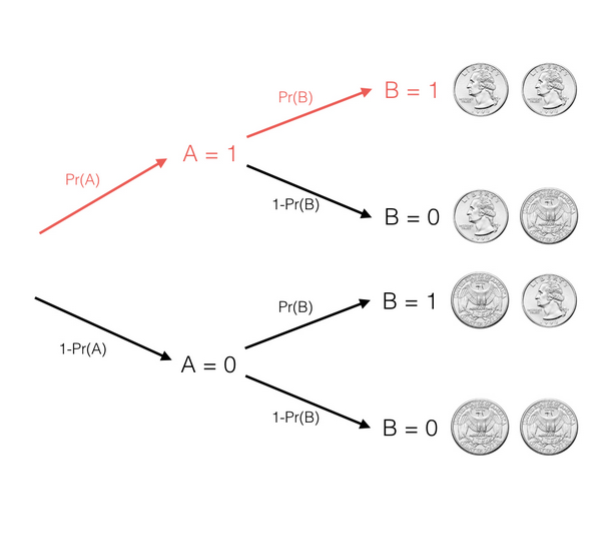
\includegraphics{image-lib/probability_of_A_and_B.png}

Consider this in terms of nested branching. First, you flip coin A with
some probability that it results in heads and some probability that it
results in tails. This branches into two possibilities: A = 1 or A = 0.
Second, you flip coin B, this causes both events to branch again
separately. Only that one branch where A and B resulted in 1 (or heads)
counts as A and B. We represent that by multiplying those two
probabilities to represent the probability of using one branch after the
other.

\begin{quote}
The probability of A and B is the probability of A times the probability
of B.
\end{quote}

Note that this is true only if events A and B appear independent i.e.~if
the result of A doesn't affect the probability of B. This is generally
true of two different coin flips and of all the cases we'll examine in
this chapter.

Two events A and B are independent if

\[\textrm{P(A and B)} = P(A) \cdot P(B)\]

and we write \(A \amalg B\). A set of events \(A_i : i \in I\) is
independent if

\[P\Bigg(\displaystyle\bigcap_{i \in J}A_i\Bigg) = \prod_{i \in J}P(A_i)\]

for every finite subset J of \emph{I}. if A and B are not independent,
we write

\[A \not\!\perp\!\!\!\perp B\]

\hypertarget{simulating-two-coins}{%
\subsection{Simulating two coins}\label{simulating-two-coins}}

To confirm this, let's try a simulation of many coin flips.

\begin{Shaded}
\begin{Highlighting}[]
\NormalTok{A <-}\StringTok{ }\KeywordTok{rbinom}\NormalTok{(}\DecValTok{100000}\NormalTok{, }\DecValTok{1}\NormalTok{, }\FloatTok{0.5}\NormalTok{)}
\end{Highlighting}
\end{Shaded}

Notice that we've set the parameters so that each draw has only one flip
and each flip has a 50\% chance of been heads. We can then simulate a
100000 flips of coin B seperately.

\begin{Shaded}
\begin{Highlighting}[]
\NormalTok{B <-}\StringTok{ }\KeywordTok{rbinom}\NormalTok{(}\DecValTok{100000}\NormalTok{, }\DecValTok{1}\NormalTok{, }\FloatTok{0.5}\NormalTok{)}
\end{Highlighting}
\end{Shaded}

Once, we have all the flips we can then compare all the pairs of them.
\texttt{R} let's us compare them with the \texttt{\&} operator and
results in \texttt{TRUE} \emph{if and only if} both A and B are 1. We
thus get a sequence of TRUEs and FALSEs for each of the 100000 pairs.
Once, we have this we can take the mean to find out the percentage that
are TRUE just as we did in the simulations in the last chapter.

\begin{Shaded}
\begin{Highlighting}[]
\KeywordTok{mean}\NormalTok{(A }\OperatorTok{&}\StringTok{ }\NormalTok{B)}
\CommentTok{#> [1] 0.25026}
\end{Highlighting}
\end{Shaded}

In this case, we see that A and B were both TRUE in about 25\% of the
simulations. This is the probability that two fair coins will bth result
in heads. This confirms our rule:

\[\textrm{P(A and B)} = P(A) \cdot P(B)\]

OR

\[\textrm{P(A and B)} = 0.5 \cdot 0.5 = 0.25\]

We could the same simulation approach if the coin weren't fair i.e.~if A
and B do not have the same probability. For example, we can set event A
to have a 10\% probability and event B to have a 70\% probability by
setting the third argument of \texttt{rbinom()} to 0.1 and 0.7
respectively. When we then combine A and B, we see that about 7\% of the
pairs are both TRUE.

\begin{Shaded}
\begin{Highlighting}[]
\NormalTok{A <-}\StringTok{ }\KeywordTok{rbinom}\NormalTok{(}\DecValTok{100000}\NormalTok{, }\DecValTok{1}\NormalTok{, }\FloatTok{0.1}\NormalTok{)}
\NormalTok{B <-}\StringTok{ }\KeywordTok{rbinom}\NormalTok{(}\DecValTok{100000}\NormalTok{, }\DecValTok{1}\NormalTok{, }\FloatTok{0.7}\NormalTok{)}
\KeywordTok{mean}\NormalTok{(A }\OperatorTok{&}\StringTok{ }\NormalTok{B)}
\CommentTok{#> [1] 0.07081}
\end{Highlighting}
\end{Shaded}

This again matches what we'll expect: The probability of

\[\textrm{P(A and B)} = 0.1 \cdot 0.7 = 0.07\]

\hypertarget{simulating-the-probability-of-a-and-b}{%
\subsection{Simulating the probability of A and
B}\label{simulating-the-probability-of-a-and-b}}

\begin{Shaded}
\begin{Highlighting}[]
\CommentTok{# Simulate 100,000 flips of a coin with a 40% chance of heads}
\NormalTok{A <-}\StringTok{ }\KeywordTok{rbinom}\NormalTok{(}\DecValTok{100000}\NormalTok{, }\DecValTok{1}\NormalTok{, }\FloatTok{0.4}\NormalTok{)}

\CommentTok{# Simulate 100,000 flips of a coin with a 20% chance of heads}
\NormalTok{B <-}\StringTok{ }\KeywordTok{rbinom}\NormalTok{(}\DecValTok{100000}\NormalTok{, }\DecValTok{1}\NormalTok{, }\FloatTok{0.2}\NormalTok{)}

\CommentTok{# Estimate the probability both A and B are heads}
\KeywordTok{mean}\NormalTok{(A }\OperatorTok{&}\StringTok{ }\NormalTok{B)}
\CommentTok{#> [1] 0.07988}
\end{Highlighting}
\end{Shaded}

\hypertarget{simulating-the-probability-of-a-b-and-c}{%
\subsection{Simulating the probability of A, B, and
C}\label{simulating-the-probability-of-a-b-and-c}}

\begin{Shaded}
\begin{Highlighting}[]
\CommentTok{# You've already simulated 100,000 flips of coins A and B}
\NormalTok{A <-}\StringTok{ }\KeywordTok{rbinom}\NormalTok{(}\DecValTok{100000}\NormalTok{, }\DecValTok{1}\NormalTok{, }\FloatTok{.4}\NormalTok{)}
\NormalTok{B <-}\StringTok{ }\KeywordTok{rbinom}\NormalTok{(}\DecValTok{100000}\NormalTok{, }\DecValTok{1}\NormalTok{, }\FloatTok{.2}\NormalTok{)}

\CommentTok{# Simulate 100,000 flips of coin C (70% chance of heads)}
\NormalTok{C <-}\StringTok{ }\KeywordTok{rbinom}\NormalTok{(}\DecValTok{100000}\NormalTok{, }\DecValTok{1}\NormalTok{, }\FloatTok{.7}\NormalTok{)}

\CommentTok{# Estimate the probability A, B, and C are all heads}
\KeywordTok{mean}\NormalTok{(A }\OperatorTok{&}\StringTok{ }\NormalTok{B }\OperatorTok{&}\StringTok{ }\NormalTok{C)}
\CommentTok{#> [1] 0.05655}
\end{Highlighting}
\end{Shaded}

\hypertarget{probability-of-a-or-b}{%
\subsection{Probability of A or B}\label{probability-of-a-or-b}}

Suppose we flip a coin twice, what is the probability that \emph{at
least one} of the flips is heads? You can imagine this as two
overlapping circles in a venn diagram? One circle represents whether
event A happened such as the first flip being heads and one whether B
happens such as the second flip being heads. The probability that either
happens is the total region.
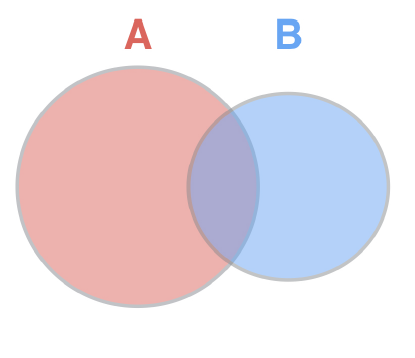
\includegraphics{image-lib/probability_of_A_or_B.png}

To find that overall probability you could start by adding up the areas
of the two circles but then you'll be double the region they overlap so
you have to substract that as well. This means:

\[P\textrm{(A or B)} = P(A) + P(B) - P\textrm{(A and B)}\]

In the last lesson you learned that as long as the event are independent

\[P\textrm{(A or B)} = P(A) + P(B) - P(A) \cdot P(B)\]

So, if A and B are independent flips of a fair coin we can take the
probability of the first being heads (50\%) plus the probability of the
second being heads (50\%) and then substract that from the probability
they both are heads.

\[P\textrm{(A or B)} = .5 + .5 - .5 \cdot .5 = .75\]

Let's try this in a simulation

\begin{Shaded}
\begin{Highlighting}[]
\NormalTok{A <-}\StringTok{ }\KeywordTok{rbinom}\NormalTok{(}\DecValTok{100000}\NormalTok{, }\DecValTok{1}\NormalTok{, }\FloatTok{.5}\NormalTok{)}
\NormalTok{B <-}\StringTok{ }\KeywordTok{rbinom}\NormalTok{(}\DecValTok{100000}\NormalTok{, }\DecValTok{1}\NormalTok{, }\FloatTok{.5}\NormalTok{)}
\KeywordTok{mean}\NormalTok{(A }\OperatorTok{|}\StringTok{ }\NormalTok{B)}
\CommentTok{#> [1] 0.74896}
\end{Highlighting}
\end{Shaded}

Here you can see the number is about 75\%; this matches the number we
earlier got from our rule. This also works if our coins are biased.

\begin{Shaded}
\begin{Highlighting}[]
\NormalTok{A <-}\StringTok{ }\KeywordTok{rbinom}\NormalTok{(}\DecValTok{100000}\NormalTok{, }\DecValTok{1}\NormalTok{, }\FloatTok{.2}\NormalTok{)}
\NormalTok{B <-}\StringTok{ }\KeywordTok{rbinom}\NormalTok{(}\DecValTok{100000}\NormalTok{, }\DecValTok{1}\NormalTok{, }\FloatTok{.6}\NormalTok{)}
\KeywordTok{mean}\NormalTok{(A }\OperatorTok{|}\StringTok{ }\NormalTok{B)}
\CommentTok{#> [1] 0.68024}
\end{Highlighting}
\end{Shaded}

We can get the same answer using the rule:

\[P\textrm{(A or B)} = .2 + .6 - .2 \cdot .6 = .68\]

One advantage of simulation approach is that it extends the cases where
mathematical solutions will get cumbersome. For example, what if we have
three coins, A, B, and C and we want to know the probability that any of
the three of them is heads i.e.~\(P\textrm{(A or B or C}\). The formular
for three events is a bit complicated and you don't need to memorize it.

\[P\textrm{(A or B or C)} = P(A) + P(B) + P(C) - P\textrm{(A and B)} \\ - P\textrm{(A and C)} - P\textrm{(B and C)} \\+ P\textrm{(A and B and C)} \]

But if you simulate the events A, B, and C, you can simply combine all
of them using the \texttt{mean()} function with the \texttt{\textbar{}}
(logical OR) operator. You can do this even with 4 or 5 events.

\hypertarget{solving-for-probability-of-a-or-b}{%
\subsection{Solving for probability of A or
B}\label{solving-for-probability-of-a-or-b}}

\[P\textrm{(A or B)} = .6 + .1 - .6 \cdot .1 = .64\]

\hypertarget{simulating-probability-of-a-or-b}{%
\subsection{Simulating probability of A or
B}\label{simulating-probability-of-a-or-b}}

\begin{Shaded}
\begin{Highlighting}[]
\CommentTok{# Simulate 100,000 flips of a coin with a 60% chance of heads}
\NormalTok{A <-}\StringTok{ }\KeywordTok{rbinom}\NormalTok{(}\DecValTok{100000}\NormalTok{, }\DecValTok{1}\NormalTok{, }\FloatTok{.6}\NormalTok{)}

\CommentTok{# Simulate 100,000 flips of a coin with a 10% chance of heads}
\NormalTok{B <-}\StringTok{ }\KeywordTok{rbinom}\NormalTok{(}\DecValTok{100000}\NormalTok{, }\DecValTok{1}\NormalTok{, }\FloatTok{.1}\NormalTok{)}

\CommentTok{# Estimate the probability either A or B is heads}
\KeywordTok{mean}\NormalTok{(A }\OperatorTok{|}\StringTok{ }\NormalTok{B)}
\CommentTok{#> [1] 0.64034}
\end{Highlighting}
\end{Shaded}

\hypertarget{probability-either-variable-is-less-than-or-equal-to-4}{%
\subsection{Probability either variable is less than or equal to
4}\label{probability-either-variable-is-less-than-or-equal-to-4}}

Suppose X is a random Binom(10, .6) variable (10 flips of a coin with
60\% chance of heads) and Y is a random Binom(10, .7) variable (10 flips
of a coin with a 70\% chance of heads), and they are independent.

What is the probability that either of the variables is less than or
equal to 4?

\begin{Shaded}
\begin{Highlighting}[]
\CommentTok{# Use rbinom to simulate 100,000 draws from each of X and Y}
\NormalTok{X <-}\StringTok{ }\KeywordTok{rbinom}\NormalTok{(}\DecValTok{100000}\NormalTok{, }\DecValTok{10}\NormalTok{, }\FloatTok{.6}\NormalTok{)}
\NormalTok{Y <-}\StringTok{ }\KeywordTok{rbinom}\NormalTok{(}\DecValTok{100000}\NormalTok{, }\DecValTok{10}\NormalTok{, }\FloatTok{.7}\NormalTok{)}

\CommentTok{# Estimate the probability either X or Y is <= to 4}
\KeywordTok{mean}\NormalTok{(X }\OperatorTok{<=}\StringTok{ }\DecValTok{4} \OperatorTok{|}\StringTok{ }\NormalTok{Y }\OperatorTok{<=}\StringTok{ }\DecValTok{4}\NormalTok{)}
\CommentTok{#> [1] 0.20478}

\CommentTok{# Use pbinom to calculate the probabilities separately}
\NormalTok{prob_X_less <-}\StringTok{ }\KeywordTok{pbinom}\NormalTok{(}\DecValTok{4}\NormalTok{, }\DecValTok{10}\NormalTok{, }\FloatTok{.6}\NormalTok{)}
\NormalTok{prob_Y_less <-}\StringTok{ }\KeywordTok{pbinom}\NormalTok{(}\DecValTok{4}\NormalTok{, }\DecValTok{10}\NormalTok{, }\FloatTok{.7}\NormalTok{)}

\CommentTok{# Combine these to calculate the exact probability either <= 4}
\NormalTok{prob_X_less }\OperatorTok{+}\StringTok{ }\NormalTok{prob_Y_less }\OperatorTok{-}\StringTok{ }\NormalTok{prob_X_less }\OperatorTok{*}\StringTok{ }\NormalTok{prob_Y_less}
\CommentTok{#> [1] 0.2057164}
\end{Highlighting}
\end{Shaded}

\hypertarget{multiplying-random-variables}{%
\subsection{Multiplying random
variables}\label{multiplying-random-variables}}

Imagine I flip this fair coin 10 times and count the number of heads,
then I take that number and triple it. What could you tell me about the
resulting number? You don't exactly what it is but could you tell me its
mean or its variance? Just like there are laws of probability for
combining events. There are laws for manipulating random variables. In
these next lessons, we'll learn to multiply random variables with a
constant or combine them together.

Suppose X is a random variable containing the result of flipping a fair
coin 10 times, we could take draws from X. One draw could be 5 another
could be 7 and yet another could be 4---each representing 10 flips of a
coin. In probability it is important to get into the habit of
manipulating random variables kind of if they are like algebraic
symbols.

\[X \sim \texttt{Binomial}(10, .5)\]

So, we could imagine defining a new random variable Y, which is 3 times
X. If X were 5, Y will be 15, and if X were 7, Y will be 21.

\[ Y \sim 3 \cdot X\]

Now, we want to know the properties of Y such as its expected value and
variance. To do that imagine a histogram of X and compare it to a
histogram of X * 3 = Y. Notice that the shape of Y is the same, but it
is larger and more spread out. So, we'll expect both the expected value
and variance to increase.

Let's see what the exact effect of multiplying by 3 is through
simulation. Try taking 100000 draws from X---a binomial with 10 flips of
a fair coin. We can take the mean and check that the expect value is
about 5 i.e.~10 flips multiplied by the probability of 0.5.

\begin{Shaded}
\begin{Highlighting}[]
\NormalTok{X <-}\StringTok{ }\KeywordTok{rbinom}\NormalTok{(}\DecValTok{100000}\NormalTok{, }\DecValTok{10}\NormalTok{, }\FloatTok{0.5}\NormalTok{)}
\KeywordTok{mean}\NormalTok{(X)}
\CommentTok{#> [1] 4.99863}
\end{Highlighting}
\end{Shaded}

To get a sample from Y, we multiply our sample of X by 3. Note: 3 * X
will multiply every individual value by 3. So we went from a 100000
draws from X to a 100000 draws from Y. We can find the expected value of
Y by taking the \texttt{mean()} and we see that it is about 15. Thus,
when we multiply a random variable by 3 we also multiply the expected
value by 3. This makes sense because we can see that the distribution
has roughly the same shape, it's just three times larger. This is a
general rule. When you multiply a random variable by a constant
\emph{k}, you also multiply the expected value by \emph{k}.

\begin{Shaded}
\begin{Highlighting}[]
\NormalTok{Y <-}\StringTok{ }\DecValTok{3} \OperatorTok{*}\StringTok{ }\NormalTok{X}
\KeywordTok{mean}\NormalTok{(Y)}
\CommentTok{#> [1] 14.99589}
\end{Highlighting}
\end{Shaded}

We can also examine what happens to the variance. The variance of X is
about 2.5. Recall that variance is size * p * 1 - p.~Now, when we
multiply it by 3 to get Y, the variance is about 22.5. It increase by a
factor of 9. Why is it 9 because that's 3\textsuperscript{2}.

\begin{Shaded}
\begin{Highlighting}[]
\KeywordTok{var}\NormalTok{(X)}
\CommentTok{#> [1] 2.488533}
\KeywordTok{var}\NormalTok{(Y)}
\CommentTok{#> [1] 22.3968}
\end{Highlighting}
\end{Shaded}

Variance is the average square distance of values from the mean. So,
when the distribution became three times wider, the variance increases
by 9. This gives two general rules for the properties of random
variables when they are multiplied by a constant.

\[E[k \cdot Y] = k \cdot E[X] \\ \textrm{Var}[k \cdot X] = k^2 \cdot \textrm{Var}[X]\]

You are learning about the application of these rules with respect to a
binomial distribution, but these holds regardless of what the
distribution the random variables follows. So, they are useful in many
applications of probability.

\hypertarget{simulating-multiplying-a-random-variable}{%
\subsection{Simulating multiplying a random
variable}\label{simulating-multiplying-a-random-variable}}

\begin{Shaded}
\begin{Highlighting}[]
\CommentTok{# Simulate 100,000 draws of a binomial with size 20 and p = .1}
\NormalTok{X <-}\StringTok{ }\KeywordTok{rbinom}\NormalTok{(}\DecValTok{100000}\NormalTok{, }\DecValTok{20}\NormalTok{, }\FloatTok{.1}\NormalTok{)}

\CommentTok{# Estimate the expected value of X}
\KeywordTok{mean}\NormalTok{(X)}
\CommentTok{#> [1] 2.00339}

\CommentTok{# Estimate the expected value of 5 * X}
\KeywordTok{mean}\NormalTok{ (}\DecValTok{5} \OperatorTok{*}\StringTok{ }\NormalTok{X)}
\CommentTok{#> [1] 10.01695}
\end{Highlighting}
\end{Shaded}

\hypertarget{variance-of-a-multiplied-random-variable}{%
\subsection{Variance of a multiplied random
variable}\label{variance-of-a-multiplied-random-variable}}

In the last exercise you simulated X from a binomial with size 20 and p
= .1 and now you'll use this same simulation to explore the variance.

\begin{Shaded}
\begin{Highlighting}[]
\CommentTok{# X is simulated from 100,000 draws of a binomial with size 20 and p = .1}
\NormalTok{X <-}\StringTok{ }\KeywordTok{rbinom}\NormalTok{(}\DecValTok{100000}\NormalTok{, }\DecValTok{20}\NormalTok{, }\FloatTok{.1}\NormalTok{)}

\CommentTok{# Estimate the variance of X}
\KeywordTok{var}\NormalTok{(X)}
\CommentTok{#> [1] 1.809691}

\CommentTok{# Estimate the variance of 5 * X}
\KeywordTok{var}\NormalTok{(}\DecValTok{5} \OperatorTok{*}\StringTok{ }\NormalTok{X)}
\CommentTok{#> [1] 45.24227}
\end{Highlighting}
\end{Shaded}

\hypertarget{adding-two-random-variables-together}{%
\subsection{Adding two random variables
together}\label{adding-two-random-variables-together}}

In the last lesson you learned how to multiply a variable by a constant.
Now, you will learn how to add multiple random variables together.
Suppose we define two random variables, X and Y. X is the result of
flipping 10 coins with each having a probability of heads of .5. Y is
the result of flipping 100 coins with each coin having a probability of
heads of .2. Assume these are two independent random variables i.e.~you
flip the coins separately. Now suppose we add those two random variables
together to get a random variable Z. If we get 6 heads in X and 22 in Y
then Z will be equal to 28.

\[X \sim \texttt{Binomial}(10, .5) \\ Y \sim \textrm{Binomial}(100, .2) \\ Z \sim X + Y\]

\begin{Shaded}
\begin{Highlighting}[]
\NormalTok{X <-}\StringTok{ }\KeywordTok{rbinom}\NormalTok{(}\DecValTok{100000}\NormalTok{, }\DecValTok{10}\NormalTok{, }\FloatTok{.5}\NormalTok{); }\KeywordTok{mean}\NormalTok{(X)}
\CommentTok{#> [1] 5.00034}
\NormalTok{Y <-}\StringTok{ }\KeywordTok{rbinom}\NormalTok{(}\DecValTok{100000}\NormalTok{, }\DecValTok{100}\NormalTok{, }\FloatTok{.2}\NormalTok{); }\KeywordTok{mean}\NormalTok{(Y)}
\CommentTok{#> [1] 20.00652}
\NormalTok{Z <-}\StringTok{ }\NormalTok{X }\OperatorTok{+}\StringTok{ }\NormalTok{Y; }\KeywordTok{mean}\NormalTok{(Z)}
\CommentTok{#> [1] 25.00686}

\KeywordTok{gf_histogram}\NormalTok{( }\OperatorTok{~}\StringTok{ }\NormalTok{X, }\DataTypeTok{bins =} \DecValTok{10}\NormalTok{, }
              \DataTypeTok{color =} \StringTok{"orange"}\NormalTok{, }
              \DataTypeTok{fill =} \StringTok{"navy blue"}\NormalTok{, }
              \DataTypeTok{xlab =} \StringTok{"X"}\NormalTok{)}
\end{Highlighting}
\end{Shaded}

\includegraphics{foundations_of_probability_in_r_files/figure-latex/unnamed-chunk-29-1.pdf}

\begin{Shaded}
\begin{Highlighting}[]
\KeywordTok{gf_histogram}\NormalTok{( }\OperatorTok{~}\StringTok{ }\NormalTok{Y, }\DataTypeTok{bins =} \DecValTok{20}\NormalTok{, }
              \DataTypeTok{color =} \StringTok{"orange"}\NormalTok{, }
              \DataTypeTok{fill =} \StringTok{"navy blue"}\NormalTok{, }
              \DataTypeTok{xlab =} \StringTok{"Y"}\NormalTok{)}
\end{Highlighting}
\end{Shaded}

\includegraphics{foundations_of_probability_in_r_files/figure-latex/unnamed-chunk-29-2.pdf}

\begin{Shaded}
\begin{Highlighting}[]
\KeywordTok{gf_histogram}\NormalTok{( }\OperatorTok{~}\StringTok{ }\NormalTok{Z, }\DataTypeTok{bins =} \DecValTok{40}\NormalTok{, }
              \DataTypeTok{color =} \StringTok{"orange"}\NormalTok{, }
              \DataTypeTok{fill =} \StringTok{"navy blue"}\NormalTok{, }
              \DataTypeTok{xlab =} \StringTok{"Z = X + Y"}\NormalTok{)}
\end{Highlighting}
\end{Shaded}

\includegraphics{foundations_of_probability_in_r_files/figure-latex/unnamed-chunk-29-3.pdf}

Notice that Z is larger and more spread out than X and Y. While the
distribution looks somewhat similar to X and Y, Z doesn't follow a
binomial distribution, but we can stll make some predictions about its
properties. We can simulate Z to find out its properties. Notice that
the expected value of X, Y, and Z is about 5, 20, and 25. This is a
general rule: The expected value of X + Y is the expected value of X
plus the expected value of Y.

\[E[X + Y] = E[X] + E[Y] \]

What about the variance of Z? We see in the histogram that it is more
spread out that either X or Y.

\begin{Shaded}
\begin{Highlighting}[]
\NormalTok{X <-}\StringTok{ }\KeywordTok{rbinom}\NormalTok{(}\DecValTok{100000}\NormalTok{, }\DecValTok{10}\NormalTok{, }\FloatTok{.5}\NormalTok{); }\KeywordTok{var}\NormalTok{(X)}
\CommentTok{#> [1] 2.496705}
\NormalTok{Y <-}\StringTok{ }\KeywordTok{rbinom}\NormalTok{(}\DecValTok{100000}\NormalTok{, }\DecValTok{100}\NormalTok{, }\FloatTok{.2}\NormalTok{); }\KeywordTok{var}\NormalTok{(Y)}
\CommentTok{#> [1] 15.97936}
\NormalTok{Z <-}\StringTok{ }\NormalTok{X }\OperatorTok{+}\StringTok{ }\NormalTok{Y; }\KeywordTok{var}\NormalTok{(Z)}
\CommentTok{#> [1] 18.4951}
\end{Highlighting}
\end{Shaded}

Notice that the variance of X, Y, and Z is about 2.5, 16, and 18.5
respectively. This also follows a general rule: the variance of the sum
of two independent random variables is the sum of their variances.

\[Var[X + Y] = Var[X] + Var[Y] \]

The rule for the addition of the expected values of two random events
still holds even if the events are not independent i.e.~even if the
outcome of one influences the outcome of the probabilities of the other.
However, the rule for adding the variances is true \emph{if only if} the
probability of each events are independent of each other.

\begin{Shaded}
\begin{Highlighting}[]
\CommentTok{# Simulate 100,000 draws of X (size 20, p = .3) and Y (size 40, p = .1)}
\NormalTok{X <-}\StringTok{ }\KeywordTok{rbinom}\NormalTok{(}\DecValTok{100000}\NormalTok{, }\DecValTok{20}\NormalTok{, }\FloatTok{.3}\NormalTok{)}
\NormalTok{Y <-}\StringTok{ }\KeywordTok{rbinom}\NormalTok{(}\DecValTok{100000}\NormalTok{, }\DecValTok{40}\NormalTok{, }\FloatTok{.1}\NormalTok{)}

\CommentTok{# Estimate the expected value of X + Y}
\KeywordTok{mean}\NormalTok{(X }\OperatorTok{+}\StringTok{ }\NormalTok{Y)}
\CommentTok{#> [1] 9.99678}
\end{Highlighting}
\end{Shaded}

\begin{Shaded}
\begin{Highlighting}[]
\CommentTok{# Simulation from last exercise of 100,000 draws from X and Y}
\NormalTok{X <-}\StringTok{ }\KeywordTok{rbinom}\NormalTok{(}\DecValTok{100000}\NormalTok{, }\DecValTok{20}\NormalTok{, }\FloatTok{.3}\NormalTok{) }
\NormalTok{Y <-}\StringTok{ }\KeywordTok{rbinom}\NormalTok{(}\DecValTok{100000}\NormalTok{, }\DecValTok{40}\NormalTok{, }\FloatTok{.1}\NormalTok{)}

\CommentTok{# Find the variance of X + Y}
\KeywordTok{var}\NormalTok{(X }\OperatorTok{+}\StringTok{ }\NormalTok{Y)}
\CommentTok{#> [1] 7.702913}

\CommentTok{# Find the variance of 3 * X + Y}
\KeywordTok{var}\NormalTok{(}\DecValTok{3} \OperatorTok{*}\StringTok{ }\NormalTok{X }\OperatorTok{+}\StringTok{ }\NormalTok{Y)}
\CommentTok{#> [1] 41.18169}
\end{Highlighting}
\end{Shaded}

\begin{quote}
Great simulating! Remember this rule only works when X and Y are
independent.
\end{quote}

\hypertarget{bayesian-statistics}{%
\section{Bayesian Statistics}\label{bayesian-statistics}}

Throughout this course we've been talking about biased coins---coins
that have a probability of heads that isn't 50\%. That knowledge is
going to come in handy because I'm worried I could have a biased coin
here. My friend Nick and I made a bet on this coin: heads I pay him;
tails he pays me. It's Nick's coin though and I am not sure I trust him,
because I think he might have given me a trick coin that comes up heads
75\% of the the time. How can we tell whether this coin is fair or
biased? Well, we can run an experiment. Suppose, we flipped a coin 20
times and we see 14 heads and 6 tails. Now, that we've seen that. Do we
believe the coin is fair or biased and could we give a probability. We
are describing the process of \emph{updating our beliefs after seeing
evidence}, which is that heart of \textbf{Bayesian statistics}.

In this chapter we'll talk about Bayesian statistics in terms of
determining whether the coin is fair or biased based on evidence. Let's
imagine that before we ran the experiment we think that there is a
chance this coin is fair and 50\% it's biased. Picture that as two piles
of coins---one of 50,000 fair coins and one of 50,000 biased coins.
Imagine that you took every coin from each of the two piles flipped it
20 times and recorded the results. You would get two histograms like
this
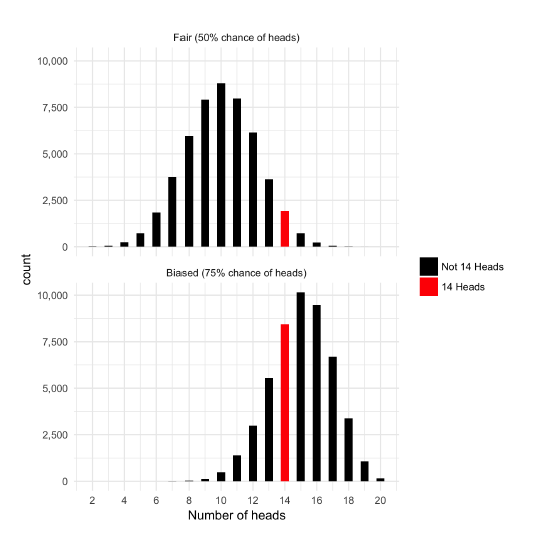
\includegraphics{image-lib/a_distribution_of_fair_and_biased_coins.png}

One for the fair coins and one for the biased coins.

Here is the trick of Bayesian statistics: When we see 14 heads out of 20
and we know whether it's either a fair or biased coin, we know that we
are in one of those red bars in the histogram, all we need to know is
which. Let's run this as a simulation.

\begin{enumerate}
\def\labelenumi{\arabic{enumi}.}
\tightlist
\item
  Go to every coin in the 50,000 fair coin flips it 20 times and record
  the number of heads. Then, we find out how many were 14s. There were
  nearly 2000 coins that resulted in 14 heads so it is possible to get
  that from a fair coin.
\end{enumerate}

\begin{Shaded}
\begin{Highlighting}[]
\NormalTok{fair <-}\StringTok{ }\KeywordTok{rbinom}\NormalTok{(}\DecValTok{50000}\NormalTok{, }\DecValTok{20}\NormalTok{, }\FloatTok{.5}\NormalTok{)}
\KeywordTok{sum}\NormalTok{(fair }\OperatorTok{==}\StringTok{ }\DecValTok{14}\NormalTok{)}
\CommentTok{#> [1] 1918}
\end{Highlighting}
\end{Shaded}

\begin{Shaded}
\begin{Highlighting}[]
\CommentTok{# gf_histogram( ~ fair) + stat_identity(aes(sum(fair == 14)), position = "identity")}
\end{Highlighting}
\end{Shaded}

\begin{enumerate}
\def\labelenumi{\arabic{enumi}.}
\setcounter{enumi}{1}
\tightlist
\item
  We do the same to see how many biased coins produce 14 heads. Notice
  that this time we changed the probability to \texttt{.75}. The
  original were of equal size but a lot more of the biased coin is
  ending up resulting in 14 heads. Notice that the red box is a lot
  taller in the biased histogram than the fair histogram and we can add
  them to see that between the two piles there were a total of 10,334
  that resulted in 14 heads i.e.~the total of the two red bars.
\end{enumerate}

\begin{Shaded}
\begin{Highlighting}[]
\NormalTok{biased <-}\StringTok{ }\KeywordTok{rbinom}\NormalTok{(}\DecValTok{50000}\NormalTok{, }\DecValTok{20}\NormalTok{, }\FloatTok{.75}\NormalTok{)}
\KeywordTok{sum}\NormalTok{(biased }\OperatorTok{==}\StringTok{ }\DecValTok{14}\NormalTok{)}
\CommentTok{#> [1] 8510}
\end{Highlighting}
\end{Shaded}

\begin{Shaded}
\begin{Highlighting}[]
\DecValTok{1898} \OperatorTok{+}\StringTok{ }\DecValTok{8436}
\CommentTok{#> [1] 10334}

\DecValTok{8436} \OperatorTok{/}\StringTok{ }\DecValTok{10334}
\CommentTok{#> [1] 0.8163344}
\end{Highlighting}
\end{Shaded}

Now, we can get the conditional probability using the formular below:

\[
\text{P(Biased | 14 Heads)} =\\ \frac{\text{No. biased w/ 14 heads}}{\text{No. total w/ 14 heads}} \\ = \frac{\text{8436}}{\texttt{1898 + 8436}} = \text{82%}
\]

We previously thought that there was a 50\% chance that the coin was
biased i.e.~the piles were of equal size, but conditional on seeing 14
heads that probability has been updated to 82\%. If we had seen 9 heads
out of 20, which is more likely to come from a fair coin than a biased
coin, the probability would have been updated in the opposite direction.

\hypertarget{updating}{%
\subsection{Updating}\label{updating}}

Suppose you have a coin that is equally likely to be fair (50\% heads)
or biased (75\% heads). You then flip the coin 20 times and see 11
heads.

Without doing any math, which do you now think is more likely- that the
coin is fair, or that the coin is biased?

\begin{itemize}
\tightlist
\item
  Answer: More likely that the coin is fair
\end{itemize}

\hypertarget{updating-with-simulation}{%
\subsection{Updating with simulation}\label{updating-with-simulation}}

We see 11 out of 20 flips from a coin that is either fair (50\% chance
of heads) or biased (75\% chance of heads). How likely is it that the
coin is fair? Answer this by simulating 50,000 fair coins and 50,000
biased coins.

\begin{Shaded}
\begin{Highlighting}[]
\CommentTok{# Simulate 50000 cases of flipping 20 coins from fair and from biased}
\NormalTok{fair <-}\StringTok{ }\KeywordTok{rbinom}\NormalTok{(}\DecValTok{50000}\NormalTok{, }\DecValTok{20}\NormalTok{, }\FloatTok{.5}\NormalTok{)}
\NormalTok{biased <-}\StringTok{ }\KeywordTok{rbinom}\NormalTok{(}\DecValTok{50000}\NormalTok{, }\DecValTok{20}\NormalTok{, }\FloatTok{.75}\NormalTok{)}

\CommentTok{# How many fair cases, and how many biased, led to exactly 11 heads?}
\NormalTok{fair_}\DecValTok{11}\NormalTok{ <-}\StringTok{ }\KeywordTok{sum}\NormalTok{(fair }\OperatorTok{==}\StringTok{ }\DecValTok{11}\NormalTok{)}
\NormalTok{biased_}\DecValTok{11}\NormalTok{ <-}\StringTok{ }\KeywordTok{sum}\NormalTok{(biased }\OperatorTok{==}\StringTok{ }\DecValTok{11}\NormalTok{)}

\CommentTok{# Find the fraction of fair coins that are 11 out of all coins that were 11}
\NormalTok{fair_}\DecValTok{11} \OperatorTok{/}\StringTok{ }\NormalTok{(fair_}\DecValTok{11} \OperatorTok{+}\StringTok{ }\NormalTok{biased_}\DecValTok{11}\NormalTok{)}
\CommentTok{#> [1] 0.8567531}
\end{Highlighting}
\end{Shaded}

\hypertarget{updating-after-16-heads}{%
\subsection{Updating after 16 heads}\label{updating-after-16-heads}}

Suppose that when you flip a different coin (that could either be fair
or biased) 20 times, you see 16 heads.

Without doing any math, which do you now think is more likely- that this
coin is fair, or that it's biased?

\begin{itemize}
\tightlist
\item
  Answer: More likely that the coin is biased.
\end{itemize}

\hypertarget{updating-with-simulation-after-16-heads}{%
\subsection{Updating with simulation after 16
heads}\label{updating-with-simulation-after-16-heads}}

We see 16 out of 20 flips from a coin that is either fair (50\% chance
of heads) or biased (75\% chance of heads). How likely is it that the
coin is fair?

\begin{Shaded}
\begin{Highlighting}[]
\CommentTok{# Simulate 50000 cases of flipping 20 coins from fair and from biased}
\NormalTok{fair <-}\StringTok{ }\KeywordTok{rbinom}\NormalTok{(}\DecValTok{50000}\NormalTok{, }\DecValTok{20}\NormalTok{, }\FloatTok{.5}\NormalTok{)}
\NormalTok{biased <-}\StringTok{ }\KeywordTok{rbinom}\NormalTok{(}\DecValTok{50000}\NormalTok{, }\DecValTok{20}\NormalTok{, }\FloatTok{.75}\NormalTok{)}

\CommentTok{# How many fair cases, and how many biased, led to exactly 16 heads?}
\NormalTok{fair_}\DecValTok{16}\NormalTok{ <-}\StringTok{ }\KeywordTok{sum}\NormalTok{(fair }\OperatorTok{==}\StringTok{ }\DecValTok{16}\NormalTok{)}
\NormalTok{biased_}\DecValTok{16}\NormalTok{ <-}\StringTok{ }\KeywordTok{sum}\NormalTok{(biased }\OperatorTok{==}\StringTok{ }\DecValTok{16}\NormalTok{)}

\CommentTok{# Find the fraction of fair coins that are 16 out of all coins that were 16}
\NormalTok{fair_}\DecValTok{16} \OperatorTok{/}\StringTok{ }\NormalTok{(fair_}\DecValTok{16} \OperatorTok{+}\StringTok{ }\NormalTok{biased_}\DecValTok{16}\NormalTok{)}
\CommentTok{#> [1] 0.02558875}
\end{Highlighting}
\end{Shaded}

\hypertarget{prior-probability}{%
\subsection{Prior probability}\label{prior-probability}}

In these exercises, we've been determining whether a coin we got from
Nick is fair or biased. We've treated as if before we saw any flips
there is a 50\% chance the coin is fair and a 50\% chance the coin is
biased towards heads. But let's say I generally trust Nick when he gave
me a coin, I figured he wasn't really trying to trick me, I am just
testing the coin to be completely safe. Let's say that when Nick gave me
the coin I thought there was only a 10\% chance it is biased and a 90\%
chance it is fair. This is called the \textbf{prior probability} and it
is an important part of Bayesian statistics.

Let's go back to the two piles of coins from the last lesson. One of the
piles is fair and one them is biased and we flip everyone of them 20
times. We know that Nick got his coins from one of these two piles and
by comparing the sizes of these red bars---the cases where the coin
resulted in exactly 14 heads---we were able to find the conditiona
probability. However, this time instead of having two equally size
piles, let's start with 90,000 coins in the fair pile and only 10,000
biased coins in the biased pile. This represents our prior probability
given the fair coins an advantage. Notice that in the resulting
histograms the relative height of the red bars i.e.~those with heads has
changed. In fact even though each of the fair coin individually was less
likely to result in 14 heads than a biased coin was there were more fair
coins that ended up with 14 heads than biased ones.

\begin{figure}
\centering
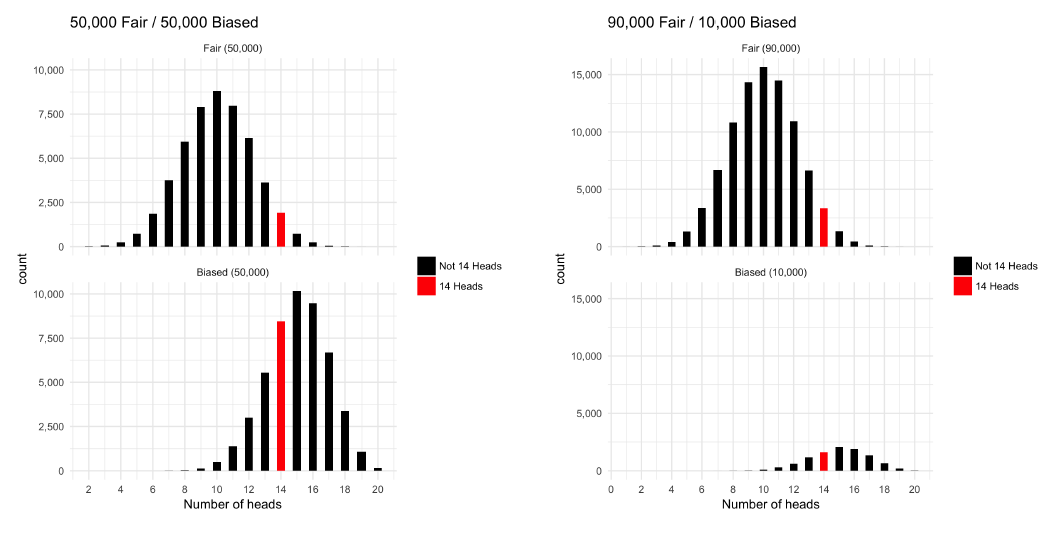
\includegraphics{image-lib/differently_sized_piles.png}
\caption{differently sized piles}
\end{figure}

We can simulate these piles to find the conditional probability that a
coin with 14 heads given our prior probability of 10\%. We first
simulate 90,000 draws from a binomial distribution where the coins are
fair. Notice that we changed the first argument (the number of draws to
90,000). We see that 3,645 of these draws resulted in 14 heads.

\begin{Shaded}
\begin{Highlighting}[]
\NormalTok{fair <-}\StringTok{ }\KeywordTok{rbinom}\NormalTok{(}\DecValTok{90000}\NormalTok{, }\DecValTok{20}\NormalTok{, }\FloatTok{.5}\NormalTok{)}
\KeywordTok{sum}\NormalTok{(fair }\OperatorTok{==}\StringTok{ }\DecValTok{14}\NormalTok{)}
\CommentTok{#> [1] 3219}
\end{Highlighting}
\end{Shaded}

We then simulate only 10,000 draws from the biased coins each with a
75\% chance of heads. We see that 1,703 of these resulted in 14 heads.

\begin{Shaded}
\begin{Highlighting}[]
\NormalTok{biased <-}\StringTok{ }\KeywordTok{rbinom}\NormalTok{(}\DecValTok{10000}\NormalTok{, }\DecValTok{20}\NormalTok{, }\FloatTok{.75}\NormalTok{)}
\KeywordTok{sum}\NormalTok{(biased }\OperatorTok{==}\StringTok{ }\DecValTok{14}\NormalTok{)}
\CommentTok{#> [1] 1650}
\end{Highlighting}
\end{Shaded}

Now, we can find out conditional probability given that we are using one
of those coins that resulted in 14 heads, what fraction of those were
biased? 33\% of them were biased. We originally thought there was a 10\%
chance the coin was biased but after seeing 14 heads out of 20 flips,
our probability has updated to 33\%.

\begin{Shaded}
\begin{Highlighting}[]
\DecValTok{1703} \OperatorTok{/}\StringTok{ }\NormalTok{(}\DecValTok{3465} \OperatorTok{+}\StringTok{ }\DecValTok{1703}\NormalTok{)}
\CommentTok{#> [1] 0.3295279}
\end{Highlighting}
\end{Shaded}

This simulation approach works even if there are more than two
possibilities for the probability of heads. For example, you can start
with three piles of coins---one that has a 25\% chance; one that has a
50\% chance; and another with 75\% chance.

\hypertarget{updating-with-priors}{%
\subsection{Updating with priors}\label{updating-with-priors}}

We see 14 out of 20 flips are heads, and start with a 80\% chance the
coin is fair and a 20\% chance it is biased to 75\%.

You'll solve this case with simulation, by starting with a ``bucket'' of
10,000 coins, where 8,000 are fair and 2,000 are biased, and flipping
each of them 20 times.

\begin{Shaded}
\begin{Highlighting}[]
\CommentTok{# Simulate 8000 cases of flipping a fair coin, and 2000 of a biased coin}
\NormalTok{fair_flips <-}\StringTok{ }\KeywordTok{rbinom}\NormalTok{(}\DecValTok{8000}\NormalTok{, }\DecValTok{20}\NormalTok{, }\FloatTok{.5}\NormalTok{)}
\NormalTok{biased_flips <-}\StringTok{ }\KeywordTok{rbinom}\NormalTok{(}\DecValTok{2000}\NormalTok{, }\DecValTok{20}\NormalTok{, }\FloatTok{.75}\NormalTok{)}

\CommentTok{# Find the number of cases from each coin that resulted in 14/20}
\NormalTok{fair_}\DecValTok{14}\NormalTok{ <-}\StringTok{ }\KeywordTok{sum}\NormalTok{(fair_flips }\OperatorTok{==}\StringTok{ }\DecValTok{14}\NormalTok{)}
\NormalTok{biased_}\DecValTok{14}\NormalTok{ <-}\StringTok{ }\KeywordTok{sum}\NormalTok{(biased_flips }\OperatorTok{==}\StringTok{ }\DecValTok{14}\NormalTok{)}

\CommentTok{# Use these to estimate the posterior probability}
\NormalTok{fair_}\DecValTok{14} \OperatorTok{/}\StringTok{ }\NormalTok{(fair_}\DecValTok{14} \OperatorTok{+}\StringTok{ }\NormalTok{biased_}\DecValTok{14}\NormalTok{)}
\CommentTok{#> [1] 0.4992224}
\end{Highlighting}
\end{Shaded}

Awesome! How did adding a prior into the mix change your outcome?

\hypertarget{updating-with-three-coins}{%
\subsection{Updating with three coins}\label{updating-with-three-coins}}

Suppose instead of a coin being either fair or biased, there are three
possibilities: that the coin is fair (50\% heads), low (25\% heads), and
high (75\% heads). There is a 80\% chance it is fair, a 10\% chance it
is biased low, and a 10\% chance it is biased high.

\begin{Shaded}
\begin{Highlighting}[]
\CommentTok{# Simulate 80,000 draws from fair coin, 10,000 from each of high and low coins}
\NormalTok{flips_fair <-}\StringTok{ }\KeywordTok{rbinom}\NormalTok{(}\DecValTok{80000}\NormalTok{, }\DecValTok{20}\NormalTok{, }\FloatTok{.5}\NormalTok{)}
\NormalTok{flips_high <-}\StringTok{ }\KeywordTok{rbinom}\NormalTok{(}\DecValTok{10000}\NormalTok{, }\DecValTok{20}\NormalTok{, }\FloatTok{.75}\NormalTok{)}
\NormalTok{flips_low <-}\StringTok{ }\KeywordTok{rbinom}\NormalTok{(}\DecValTok{10000}\NormalTok{, }\DecValTok{20}\NormalTok{, }\FloatTok{.25}\NormalTok{)}

\CommentTok{# Compute the number of coins that resulted in 14 heads from each of these piles}
\NormalTok{fair_}\DecValTok{14}\NormalTok{ <-}\StringTok{ }\KeywordTok{sum}\NormalTok{(flips_fair }\OperatorTok{==}\StringTok{ }\DecValTok{14}\NormalTok{)}
\NormalTok{high_}\DecValTok{14}\NormalTok{ <-}\StringTok{ }\KeywordTok{sum}\NormalTok{(flips_high }\OperatorTok{==}\StringTok{ }\DecValTok{14}\NormalTok{)}
\NormalTok{low_}\DecValTok{14}\NormalTok{ <-}\StringTok{ }\KeywordTok{sum}\NormalTok{(flips_low }\OperatorTok{==}\StringTok{ }\DecValTok{14}\NormalTok{)}

\CommentTok{# Compute the posterior probability that the coin was fair}
\NormalTok{fair_}\DecValTok{14} \OperatorTok{/}\StringTok{ }\NormalTok{(fair_}\DecValTok{14} \OperatorTok{+}\StringTok{ }\NormalTok{high_}\DecValTok{14} \OperatorTok{+}\StringTok{ }\NormalTok{low_}\DecValTok{14}\NormalTok{)}
\CommentTok{#> [1] 0.6381281}
\end{Highlighting}
\end{Shaded}

Wow! Great work! Adding another coin doesn't make things too much
harder, does it?

\hypertarget{bayes-theorem}{%
\subsection{Bayes' Theorem}\label{bayes-theorem}}

We've used simulation to estimate a conditional probability that a coin
is fair or biased. For example, we looked at the distribution of 90,000
fair coins and 10,000 biased coins and saw how many coins from each pile
resulted in 14 heads. We saw about 3000 resulting in heads amongst the
fair coins and about 1500 among the biased coins. But what we are really
working with in these simulations is \emph{probability densities}.
Consider the histogram in terms of the probability a coin out of the
100,000 we are flipping ends up with that outcome. In this lesson,
rather that simulating many coins to determine whether a coin is biased
we'll use a probability density specifically the \texttt{dbinom()}
function to find an exact answer. In the process we'll introduce one of
the most important equations in probability, \textbf{Bayes' Theorem}.

Recall that we use simulation to find the number of fair coins resulting
in 14 heads out of the 90,000 in the original pile. Now, rather than
simulating it with \texttt{rbinom()}, let's find the exact probability
of 14 heads with the \texttt{dbinom()} function. But notice we also
multiply it with the prior probability the coin is fair
i.e.~\textbf{0.9}. That's the equivalent of the 90,000 in the
\texttt{rbinom()}. It calculates the probability that the coin is both
fair and results in 14 heads.

\begin{Shaded}
\begin{Highlighting}[]
\NormalTok{fair <-}\StringTok{ }\KeywordTok{rbinom}\NormalTok{(}\DecValTok{90000}\NormalTok{, }\DecValTok{20}\NormalTok{, }\FloatTok{0.5}\NormalTok{)}
\KeywordTok{sum}\NormalTok{(fair }\OperatorTok{==}\StringTok{ }\DecValTok{14}\NormalTok{)}
\CommentTok{#> [1] 3330}
\end{Highlighting}
\end{Shaded}

\begin{Shaded}
\begin{Highlighting}[]
\KeywordTok{dbinom}\NormalTok{(}\DecValTok{14}\NormalTok{, }\DecValTok{20}\NormalTok{, }\FloatTok{.5}\NormalTok{) }\OperatorTok{*}\StringTok{ }\FloatTok{.9}
\CommentTok{#> [1] 0.03326797}
\end{Highlighting}
\end{Shaded}

\[\texttt{P(14 heads | Fair)} \cdot \texttt{P(Fair)}\]

We also simulated 10,000 biased coins and found the number of times
there were 14 heads out of 20 flips. We can replace that with
\texttt{dbinom()} using a .75 probability then multiplying it by the 0.1
prior probability that a coin was biased. These gets the exact
probability shown in red in the histograms.

\begin{figure}
\centering
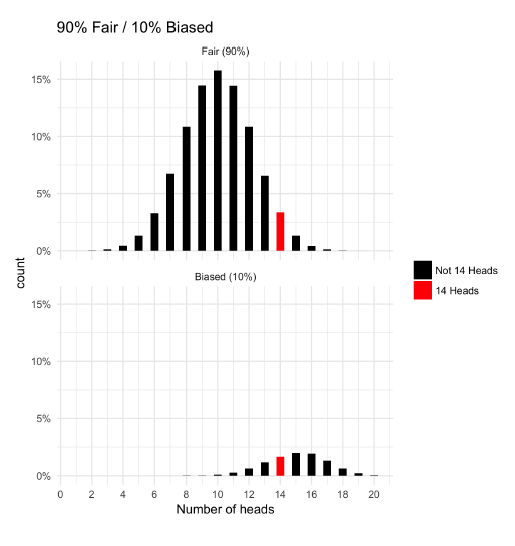
\includegraphics{image-lib/prob_densities_of_fair_and_biased_coins.png}
\caption{probability density of fair and biased coins}
\end{figure}

\begin{Shaded}
\begin{Highlighting}[]
\NormalTok{biased <-}\StringTok{ }\KeywordTok{rbinom}\NormalTok{(}\DecValTok{10000}\NormalTok{, }\DecValTok{20}\NormalTok{, }\FloatTok{.75}\NormalTok{)}
\KeywordTok{sum}\NormalTok{(biased }\OperatorTok{==}\StringTok{ }\DecValTok{14}\NormalTok{)}
\CommentTok{#> [1] 1745}
\end{Highlighting}
\end{Shaded}

\begin{Shaded}
\begin{Highlighting}[]
\KeywordTok{dbinom}\NormalTok{(}\DecValTok{14}\NormalTok{, }\DecValTok{20}\NormalTok{, }\FloatTok{.75}\NormalTok{) }\OperatorTok{*}\StringTok{ }\FloatTok{.1}
\CommentTok{#> [1] 0.01686093}
\end{Highlighting}
\end{Shaded}

\[\texttt{P(14 heads | Biased)} \cdot \texttt{P(Biased)}\]

Now, that we have these probabilities, we can combine them in the same
way we did the coins. To find the probability a coin is biased
conditional on resulting in 14 heads out of 20, we look at the
probability it is both 14 and biased out of the total probability that
it resulted in 14 heads. This is the equivalent at looking at both of
the red bars and asking which red bar the coin is in. As we did in the
last slide, we can can compute each of this probabilities by multiplying
the probabililty density by the prior propability.

\[\texttt{P(Biased | 14 Heads)} \\ = 
\frac{\texttt{P(14 Heads and Biased)}}{\texttt{P(14 Heads and Biased)} + \texttt{P(14 Heads and Fair)}} \\ = 
\frac{\texttt{P(14 Heads | Biased)P(Biased)}}{\texttt{P(14 Heads | Biased)P(Biased) + P(14 Heads | Fair)P(Fair)}} \]

In the numerator, we are multiplying the probability of biased coins
will result in 14 heads with the prior probability that the coin is
biased. You are now able to calculate this in \texttt{R} by using
\texttt{dbinom()} to calculate each of the densities multiplying each by
the prior probabilities and then putting them into a fraction.

\begin{Shaded}
\begin{Highlighting}[]
\NormalTok{prob_}\DecValTok{14}\NormalTok{_fair <-}\StringTok{ }\KeywordTok{dbinom}\NormalTok{(}\DecValTok{14}\NormalTok{, }\DecValTok{20}\NormalTok{, }\FloatTok{.5}\NormalTok{) }\OperatorTok{*}\StringTok{ }\FloatTok{.9}
\NormalTok{prob_}\DecValTok{14}\NormalTok{_biased <-}\StringTok{ }\KeywordTok{dbinom}\NormalTok{(}\DecValTok{14}\NormalTok{, }\DecValTok{20}\NormalTok{, }\FloatTok{.5}\NormalTok{) }\OperatorTok{*}\StringTok{ }\FloatTok{.1}

\NormalTok{prob_}\DecValTok{14}\NormalTok{_biased }\OperatorTok{/}\StringTok{ }\NormalTok{(prob_}\DecValTok{14}\NormalTok{_fair }\OperatorTok{+}\StringTok{ }\NormalTok{prob_}\DecValTok{14}\NormalTok{_biased)}
\CommentTok{#> [1] 0.1}
\end{Highlighting}
\end{Shaded}

This exact solution is an application of Bayes' Theorem:

\[\texttt{P(A | B)} \\ = 
\frac{\texttt{P(B | A)(P(A)}}{\texttt{P(B | A)P(A)} + \texttt{P(B | not A)P(not A)}} \\ A = \texttt{Biased} \\ B = \texttt{14 Heads}\]

Bayes' Theorem is usually written in terms of finding the probability of
in terms of finding the probability of event A given B when you know the
probability of event B given event A. In the problem we explored in this
chapter event A is the set of biased coins and event B is that it
resulted in 14 heads out of 20. This is why Bayes' Theorem was useful.
We knew the probability of getting 14 heads given that the coin is
biased, but we needed to convert it to the probability that the coin is
biased given that it resulted in 14 heads. We could have just started
the chapter with this equation, but our simulation showed with the
numerator and denominator really represents by imagining what fraction
of all coins resulting in 14 heads were biased. This will help you to
understand and apply the theorem to calculate conditional probabilities
in the future.

\hypertarget{updating-with-bayes-theorem}{%
\subsection{Updating with Bayes
Theorem}\label{updating-with-bayes-theorem}}

In this chapter, you used simulation to estimate the posterior
probability that a coin that resulted in 11 heads out of 20 is fair. Now
you'll calculate it again, this time using the exact probabilities from
\texttt{dbinom()}. There is a 50\% chance the coin is fair and a 50\%
chance the coin is biased.

\begin{Shaded}
\begin{Highlighting}[]
\CommentTok{# Use dbinom to calculate the probability of 11/20 heads with fair or biased coin}
\NormalTok{probability_fair <-}\StringTok{ }\KeywordTok{dbinom}\NormalTok{(}\DecValTok{11}\NormalTok{, }\DecValTok{20}\NormalTok{, }\FloatTok{0.5}\NormalTok{)}
\NormalTok{probability_biased <-}\StringTok{ }\KeywordTok{dbinom}\NormalTok{(}\DecValTok{11}\NormalTok{, }\DecValTok{20}\NormalTok{, }\FloatTok{0.75}\NormalTok{)}

\CommentTok{# Calculate the posterior probability that the coin is fair}
\NormalTok{probability_fair }\OperatorTok{/}\StringTok{ }\NormalTok{(probability_fair }\OperatorTok{+}\StringTok{ }\NormalTok{probability_biased)}
\CommentTok{#> [1] 0.8554755}
\end{Highlighting}
\end{Shaded}

Awesome job! Do you think calculating or simulating the answer is
easier? Which makes more sense? I like the idea of simulating the
experiment so as to get to the answer.

\hypertarget{updating-for-other-outcomes}{%
\subsection{Updating for other
outcomes}\label{updating-for-other-outcomes}}

In the last exercise, you solved for the probability that the coin is
fair if it results in 11 heads out of 20 flips, assuming that beforehand
there was an equal chance of it being a fair coin or a biased coin.
Recall that the code looked something like:

\begin{Shaded}
\begin{Highlighting}[]
\NormalTok{probability_fair <-}\StringTok{ }\KeywordTok{dbinom}\NormalTok{(}\DecValTok{11}\NormalTok{, }\DecValTok{20}\NormalTok{, }\FloatTok{.5}\NormalTok{)}
\NormalTok{probability_biased <-}\StringTok{ }\KeywordTok{dbinom}\NormalTok{(}\DecValTok{11}\NormalTok{, }\DecValTok{20}\NormalTok{, }\FloatTok{.75}\NormalTok{)}
\NormalTok{probability_fair }\OperatorTok{/}\StringTok{ }\NormalTok{(probability_fair }\OperatorTok{+}\StringTok{ }\NormalTok{probability_biased)}
\end{Highlighting}
\end{Shaded}

Now you'll find, using the \texttt{dbinom()} approach, the posterior
probability if there were two other outcomes.

\begin{Shaded}
\begin{Highlighting}[]
\CommentTok{# Find the probability that a coin resulting in 14/20 is fair}
\NormalTok{probability_fair_}\DecValTok{14}\NormalTok{ <-}\StringTok{ }\KeywordTok{dbinom}\NormalTok{(}\DecValTok{14}\NormalTok{, }\DecValTok{20}\NormalTok{, }\FloatTok{0.5}\NormalTok{)}
\NormalTok{probability_biased_}\DecValTok{14}\NormalTok{ <-}\StringTok{ }\KeywordTok{dbinom}\NormalTok{(}\DecValTok{14}\NormalTok{, }\DecValTok{20}\NormalTok{, }\FloatTok{0.75}\NormalTok{)}

\NormalTok{probability_fair_}\DecValTok{14} \OperatorTok{/}\StringTok{ }\NormalTok{(probability_fair_}\DecValTok{14} \OperatorTok{+}\StringTok{ }\NormalTok{probability_biased_}\DecValTok{14}\NormalTok{)}
\CommentTok{#> [1] 0.179811}

\CommentTok{# Find the probability that a coin resulting in 18/20 is fair}
\NormalTok{probability_fair_}\DecValTok{18}\NormalTok{ <-}\StringTok{ }\KeywordTok{dbinom}\NormalTok{(}\DecValTok{18}\NormalTok{, }\DecValTok{20}\NormalTok{, }\FloatTok{0.5}\NormalTok{)}
\NormalTok{probability_biased_}\DecValTok{18}\NormalTok{ <-}\StringTok{ }\KeywordTok{dbinom}\NormalTok{(}\DecValTok{18}\NormalTok{, }\DecValTok{20}\NormalTok{, }\FloatTok{0.75}\NormalTok{)}

\NormalTok{probability_fair_}\DecValTok{18} \OperatorTok{/}\StringTok{ }\NormalTok{(probability_fair_}\DecValTok{18} \OperatorTok{+}\StringTok{ }\NormalTok{probability_biased_}\DecValTok{18}\NormalTok{)}
\CommentTok{#> [1] 0.002699252}
\end{Highlighting}
\end{Shaded}

\hypertarget{more-updating-with-priors}{%
\subsection{More updating with priors}\label{more-updating-with-priors}}

Suppose we see 16 heads out of 20 flips, which would normally be strong
evidence that the coin is biased. However, suppose we had set a prior
probability of a 99\% chance that the coin is fair (50\% chance of
heads), and only a 1\% chance that the coin is biased (75\% chance of
heads).

You'll solve this exercise by finding the exact answer with dbinom() and
Bayes' theorem. Recall that Bayes' theorem looks like:

\[\texttt{P(fair | A)} \\ = 
\frac{\texttt{P(A | fair)(P(fair)}}{\texttt{P(A | fair)P(fair)} + \texttt{P(A | Biased)P(Biased)}}\]

\begin{Shaded}
\begin{Highlighting}[]
\CommentTok{# Use dbinom to find the probability of 16/20 from a fair or biased coin}
\NormalTok{probability_}\DecValTok{16}\NormalTok{_fair <-}\StringTok{ }\KeywordTok{dbinom}\NormalTok{(}\DecValTok{16}\NormalTok{, }\DecValTok{20}\NormalTok{, }\FloatTok{0.5}\NormalTok{) }
\NormalTok{probability_}\DecValTok{16}\NormalTok{_biased <-}\StringTok{ }\KeywordTok{dbinom}\NormalTok{(}\DecValTok{16}\NormalTok{, }\DecValTok{20}\NormalTok{, }\FloatTok{0.75}\NormalTok{) }

\CommentTok{# Use Bayes' theorem to find the posterior probability that the coin is fair}
\NormalTok{(probability_}\DecValTok{16}\NormalTok{_fair }\OperatorTok{*}\StringTok{ }\FloatTok{0.99}\NormalTok{) }\OperatorTok{/}\StringTok{ }\NormalTok{(probability_}\DecValTok{16}\NormalTok{_fair }\OperatorTok{*}\StringTok{ }\FloatTok{0.99} \OperatorTok{+}\StringTok{ }\NormalTok{probability_}\DecValTok{16}\NormalTok{_biased }\OperatorTok{*}\StringTok{ }\FloatTok{0.01}\NormalTok{)}
\CommentTok{#> [1] 0.7068775}
\end{Highlighting}
\end{Shaded}

Amazing! It seems like your choice of prior can have a pretty big effect
on the final answer.

\hypertarget{related-distributions}{%
\section{Related Distributions}\label{related-distributions}}

\hypertarget{the-normal-distribution}{%
\subsection{The Normal Distribution}\label{the-normal-distribution}}

We've been exploring the binomial distribution, the result of flipping
multiple coins multiple times and calculating the number of heads. In
this chapter, we're going to introduce three other important probability
distributions and see how they each connect to the theme of flipping
coins. You will not only add these distributions to your statistical
tool box, but also see how the principles we've learned about working
with random variables and simulation are important far beyond the
binomial.

So far, you've often looked at a binomial where each draws made up of 10
flips of a coin has a 50\% chance of heads. That will look like this
distribution: a histogram where the most common value is 5.

\begin{Shaded}
\begin{Highlighting}[]
\KeywordTok{gf_histogram}\NormalTok{( }\OperatorTok{~}\StringTok{ }\KeywordTok{rbinom}\NormalTok{(}\DecValTok{100000}\NormalTok{, }\DecValTok{10}\NormalTok{, }\FloatTok{.5}\NormalTok{), }\DataTypeTok{xlab =} \StringTok{"flips"}\NormalTok{)}
\end{Highlighting}
\end{Shaded}

\includegraphics{foundations_of_probability_in_r_files/figure-latex/unnamed-chunk-53-1.pdf}

Now imagine instead of flipping 10 or 20 fair coins in each draw we
flipped 1000. Now the distribution of the number of heads is centered
around 500. Notice the distribution is now taking on a sort of
symmetrical, bell curve shape. This is because when you draw from the
binomial with a very large size i.e.~many coin flips, the results
approximates a \textbf{normal distribution}. Approximations from one
distribution to another are important in probability since they let you
make connections between statistical tools.

\begin{Shaded}
\begin{Highlighting}[]
\KeywordTok{gf_histogram}\NormalTok{( }\OperatorTok{~}\StringTok{ }\KeywordTok{rbinom}\NormalTok{(}\DecValTok{100000}\NormalTok{, }\DecValTok{1000}\NormalTok{, }\FloatTok{.5}\NormalTok{), }\DataTypeTok{xlab =} \StringTok{"flips"}\NormalTok{)}
\end{Highlighting}
\end{Shaded}

\includegraphics{foundations_of_probability_in_r_files/figure-latex/unnamed-chunk-54-1.pdf}

You'll sometimes hear a normal distribution referred to as a
\textbf{gaussian distribution} or a \textbf{bell curve}. It's famous
because many distributions in nature take this shape such as measurement
errors in scientific experiments and because its mathematical properties
are well-understood. Many of the courses on the datacamp platform show
how the normal distribution can be used in statistical inference. While
the binomial is defined in terms of parameters \(size\) i.e.~number of
flips and \(p\), the probability of heads, the normal distribution is
defined based on two other parameters: the mean (\(\mu\)) and the
standard deviation (\(\sigma\)).

Mathematically, we usually represent the mean as the Greek letter
(\(\mu\)) and standard deviation as the Greek letter (\(\sigma\)).

\[X \sim Normal(\mu, \sigma)\]

In chapters 1 and 2, we introduced the concept of variance i.e.~the
average square distance from the mean. The standard deviation is square
root of the variance.

\[\sigma = \sqrt{Var(X)}\]

While \texttt{R} defines the normal distribution using the standard
deviation, some statisticians choose to define it using the variance.
It's not that important what you choose because if you know one you know
the other. You can square the standard deviation to get the variance or
take square root of the varianc to get the standard deviation. Because
the normal is defined in terms of the mean and standard deviation, it's
easy to find the normal approximation to a particular binomial
distribution. For example, we could a sample of a 100,000 draws in a
binomial distribution with size 1000 and probability 0.5.

\begin{Shaded}
\begin{Highlighting}[]
\NormalTok{binomial_flips <-}\StringTok{ }\KeywordTok{rbinom}\NormalTok{(}\DecValTok{100000}\NormalTok{, }\DecValTok{1000}\NormalTok{, }\FloatTok{0.5}\NormalTok{)}
\end{Highlighting}
\end{Shaded}

\[\mu = size \cdot p\]

\[\sigma = \sqrt{size \cdot p \cdot (1 - p)}\]

\begin{Shaded}
\begin{Highlighting}[]
\NormalTok{expected_value <-}\StringTok{ }\DecValTok{1000} \OperatorTok{*}\StringTok{ }\FloatTok{0.5}
\NormalTok{variance <-}\StringTok{ }\DecValTok{1000} \OperatorTok{*}\StringTok{ }\FloatTok{0.5} \OperatorTok{*}\StringTok{ }\NormalTok{(}\DecValTok{1} \OperatorTok{-}\StringTok{ }\FloatTok{0.5}\NormalTok{)}
\NormalTok{stdev <-}\StringTok{ }\KeywordTok{sqrt}\NormalTok{(variance)}
\end{Highlighting}
\end{Shaded}

We can then simulate from the normal using this parameters. We do this
with the \texttt{rnorm()} function rather than \texttt{rbinom()}. The
first argument is the number of draws, the second is the mean i.e.~the
same as the expected value of the binomial, and the third is the
standard deviation.

\begin{Shaded}
\begin{Highlighting}[]
\NormalTok{normal <-}\StringTok{ }\KeywordTok{rnorm}\NormalTok{(}\DecValTok{100000}\NormalTok{, expected_value, stdev)}
\end{Highlighting}
\end{Shaded}

Now, that we've simulated 100,000 draws from the binomial and from the
corresponding normal distribution, we'll like to compare them to see if
the normal really is a good approximation. Both of the plots look
similar confirming that the normal distribution is a good approximation
of the the binomial.

\begin{Shaded}
\begin{Highlighting}[]
\NormalTok{binomial_draws <-}\StringTok{ }\KeywordTok{data.frame}\NormalTok{(}\DataTypeTok{draws =} \KeywordTok{rbinom}\NormalTok{(}\DecValTok{100000}\NormalTok{, }\DecValTok{1000}\NormalTok{, }\FloatTok{0.5}\NormalTok{))}
\NormalTok{normal_draws <-}\StringTok{ }\KeywordTok{data.frame}\NormalTok{(}\DataTypeTok{draws =} \KeywordTok{rnorm}\NormalTok{(}\DecValTok{100000}\NormalTok{, expected_value, stdev))   }

\NormalTok{binomial_draws}\OperatorTok{$}\NormalTok{type <-}\StringTok{ 'binomial'}
\NormalTok{normal_draws}\OperatorTok{$}\NormalTok{type <-}\StringTok{ 'normal'}

\NormalTok{prob_dist <-}\StringTok{ }\KeywordTok{rbind}\NormalTok{(binomial_draws, normal_draws)}

\KeywordTok{head}\NormalTok{(prob_dist)}
\end{Highlighting}
\end{Shaded}

\begin{longtable}[]{@{}rl@{}}
\toprule
draws & type\tabularnewline
\midrule
\endhead
493 & binomial\tabularnewline
500 & binomial\tabularnewline
507 & binomial\tabularnewline
483 & binomial\tabularnewline
500 & binomial\tabularnewline
494 & binomial\tabularnewline
\bottomrule
\end{longtable}

\begin{Shaded}
\begin{Highlighting}[]

\KeywordTok{gf_histogram}\NormalTok{( }\OperatorTok{~}\StringTok{ }\NormalTok{draws, }\DataTypeTok{data =}\NormalTok{ prob_dist, }\DataTypeTok{size =} \FloatTok{0.5}\NormalTok{, }\DataTypeTok{color =} \StringTok{"orange"}\NormalTok{, }\DataTypeTok{fill =} \StringTok{"navy blue"}\NormalTok{) }\OperatorTok\StringTok{ }\KeywordTok{gf_facet_wrap}\NormalTok{(}\OperatorTok{~}\StringTok{ }\NormalTok{type)}
\end{Highlighting}
\end{Shaded}

\includegraphics{foundations_of_probability_in_r_files/figure-latex/unnamed-chunk-58-1.pdf}

\hypertarget{simulating-from-the-binomial-and-the-normal}{%
\subsection{Simulating from the binomial and the
normal}\label{simulating-from-the-binomial-and-the-normal}}

In this exercise you'll see for yourself whether the normal is a
reasonable approximation to the binomial by simulating large samples
from the binomial distribution and its normal approximation and
comparing their histograms.

\begin{Shaded}
\begin{Highlighting}[]
\CommentTok{# compare_histogram <- function(variable1, variable2) \{}
\CommentTok{#   x <- data.frame(value = variable1, variable = "Variable 1")}
\CommentTok{#   y <- data.frame(value = variable2, variable = "Variable 2")}
\CommentTok{#   ggplot(rbind(x, y), aes(value)) +}
\CommentTok{#     geom_histogram() +}
\CommentTok{#     facet_wrap(~ variable, nrow = 2)}
\CommentTok{# \}}
\end{Highlighting}
\end{Shaded}

\begin{Shaded}
\begin{Highlighting}[]
\NormalTok{compare_histograms <-}\StringTok{ }\ControlFlowTok{function}\NormalTok{(variable1, variable2) \{}
\NormalTok{  x <-}\StringTok{ }\KeywordTok{data.frame}\NormalTok{(}\DataTypeTok{value =}\NormalTok{ variable1, }\DataTypeTok{variable =} \StringTok{"Variable 1"}\NormalTok{)}
\NormalTok{  y <-}\StringTok{ }\KeywordTok{data.frame}\NormalTok{(}\DataTypeTok{value =}\NormalTok{ variable2, }\DataTypeTok{variable =} \StringTok{"Variable 2"}\NormalTok{)}
    \KeywordTok{rbind}\NormalTok{(x, y) }\OperatorTok\StringTok{ }
\StringTok{    }\NormalTok{ggformula}\OperatorTok{::}\KeywordTok{gf_histogram}\NormalTok{(}\OperatorTok{~}\StringTok{ }\NormalTok{value) }\OperatorTok\StringTok{ }
\StringTok{    }\KeywordTok{gf_facet_wrap}\NormalTok{(}\OperatorTok{~}\StringTok{ }\NormalTok{variable, }\DataTypeTok{nrow =} \DecValTok{2}\NormalTok{)}
\NormalTok{\}}
\end{Highlighting}
\end{Shaded}

\begin{Shaded}
\begin{Highlighting}[]
\CommentTok{# Draw a random sample of 100,000 from the Binomial(1000, .2) distribution}
\NormalTok{binom_sample <-}\StringTok{ }\KeywordTok{rbinom}\NormalTok{(}\DecValTok{100000}\NormalTok{, }\DecValTok{1000}\NormalTok{, }\FloatTok{0.2}\NormalTok{)}

\CommentTok{# Draw a random sample of 100,000 from the normal approximation}
\NormalTok{normal_sample <-}\StringTok{ }\KeywordTok{rnorm}\NormalTok{(}\DecValTok{100000}\NormalTok{, }\DecValTok{200}\NormalTok{, }\KeywordTok{sqrt}\NormalTok{(}\KeywordTok{var}\NormalTok{(binom_sample)))}

\CommentTok{# Compare the two distributions with the compare_histograms function}
\KeywordTok{compare_histograms}\NormalTok{(binom_sample, normal_sample)}
\end{Highlighting}
\end{Shaded}

\includegraphics{foundations_of_probability_in_r_files/figure-latex/unnamed-chunk-59-1.pdf}

\hypertarget{comparing-the-cumulative-density-of-the-binomial}{%
\subsection{Comparing the cumulative density of the
binomial}\label{comparing-the-cumulative-density-of-the-binomial}}

If you flip 1000 coins that each have a 20\% chance of being heads, what
is the probability you would get 190 heads or fewer?

You'll get similar answers if you solve this with the binomial or its
normal approximation. In this exercise, you'll solve it both ways, using
both simulation and exact calculation.

\begin{Shaded}
\begin{Highlighting}[]
\CommentTok{# Simulations from the normal and binomial distributions}
\NormalTok{binom_sample <-}\StringTok{ }\KeywordTok{rbinom}\NormalTok{(}\DecValTok{100000}\NormalTok{, }\DecValTok{1000}\NormalTok{, }\FloatTok{.2}\NormalTok{)}
\NormalTok{normal_sample <-}\StringTok{ }\KeywordTok{rnorm}\NormalTok{(}\DecValTok{100000}\NormalTok{, }\DecValTok{200}\NormalTok{, }\KeywordTok{sqrt}\NormalTok{(}\DecValTok{160}\NormalTok{))}

\CommentTok{# Use binom_sample to estimate the probability of <= 190 heads}
\KeywordTok{mean}\NormalTok{(binom_sample }\OperatorTok{<=}\StringTok{ }\DecValTok{190}\NormalTok{)}
\CommentTok{#> [1] 0.22883}

\CommentTok{# Use normal_sample to estimate the probability of <= 190 heads}
\KeywordTok{mean}\NormalTok{(normal_sample }\OperatorTok{<=}\StringTok{ }\DecValTok{190}\NormalTok{)}
\CommentTok{#> [1] 0.2159}

\CommentTok{# Calculate the probability of <= 190 heads with pbinom}
\KeywordTok{pbinom}\NormalTok{(}\DecValTok{190}\NormalTok{, }\DecValTok{1000}\NormalTok{, }\FloatTok{0.2}\NormalTok{)}
\CommentTok{#> [1] 0.2273564}

\CommentTok{# Calculate the probability of <= 190 heads with pnorm}
\KeywordTok{pnorm}\NormalTok{(}\DecValTok{190}\NormalTok{, }\DecValTok{200}\NormalTok{, }\KeywordTok{sqrt}\NormalTok{(}\DecValTok{160}\NormalTok{))}
\CommentTok{#> [1] 0.2145977}
\end{Highlighting}
\end{Shaded}

Great job! There are a lot of different ways to go about getting similar
answers.

\hypertarget{comparing-the-distributions-of-the-normal-and-binomial-for-low-n}{%
\subsection{Comparing the distributions of the normal and binomial for
low
n}\label{comparing-the-distributions-of-the-normal-and-binomial-for-low-n}}

When we flip a lot of coins, it looks like the normal distribution is a
pretty close approximation. What about when we flip only 10 coins, each
still having a 20\% chance of coming up heads? Is the normal still a
good approximation?

\begin{Shaded}
\begin{Highlighting}[]
\CommentTok{# Draw a random sample of 100,000 from the Binomial(10, .2) distribution}
\NormalTok{binom_sample <-}\StringTok{ }\KeywordTok{rbinom}\NormalTok{(}\DecValTok{100000}\NormalTok{, }\DecValTok{10}\NormalTok{, }\FloatTok{0.2}\NormalTok{)}

\CommentTok{# Draw a random sample of 100,000 from the normal approximation}
\NormalTok{normal_sample <-}\StringTok{ }\KeywordTok{rnorm}\NormalTok{(}\DecValTok{100000}\NormalTok{, }\DecValTok{2}\NormalTok{, }\KeywordTok{sqrt}\NormalTok{(}\FloatTok{1.6}\NormalTok{))}

\CommentTok{# Compare the two distributions with the compare_histograms function}
\KeywordTok{compare_histograms}\NormalTok{(binom_sample, normal_sample)}
\end{Highlighting}
\end{Shaded}

\includegraphics{foundations_of_probability_in_r_files/figure-latex/unnamed-chunk-61-1.pdf}

Good work! How do the sample size and the probability of success effect
the accuracy of the normal approximation?

\begin{itemize}
\tightlist
\item
  Answer: We need a larger sample size in order for the normal
  distribution to approximate the binomial distribution.
\end{itemize}

\hypertarget{the-poisson-distribution}{%
\subsection{The Poisson Distribution}\label{the-poisson-distribution}}

In the last lesson we tried flipping a very large number of coins and we
noticed the resulting number of heads could be approximately by a normal
distribution. In this lesson we'll introduce another distribution that
is related to the binomial, the poisson distribution. Suppose we flip
1000 coins but this time every coin has only a 1 / 1000 probability of
being heads. We are considering \emph{how often a rare event happens out
of a large number of opportunities}. We can simulate this with the
\texttt{rbinom()} function by setting the second parameter to a 1000 and
the third to be 1 / 1000.

\begin{Shaded}
\begin{Highlighting}[]
\NormalTok{binomial_flips <-}\StringTok{ }\KeywordTok{rbinom}\NormalTok{(}\DecValTok{100000}\NormalTok{, }\DecValTok{1000}\NormalTok{, }\DecValTok{1} \OperatorTok{/}\StringTok{ }\DecValTok{1000}\NormalTok{)}
\end{Highlighting}
\end{Shaded}

The histogram will look like this:

\begin{Shaded}
\begin{Highlighting}[]
\KeywordTok{gf_histogram}\NormalTok{( }\OperatorTok{~}\StringTok{ }\NormalTok{binomial_flips, }\DataTypeTok{xlab =} \StringTok{"flips"}\NormalTok{)}
\end{Highlighting}
\end{Shaded}

\includegraphics{foundations_of_probability_in_r_files/figure-latex/unnamed-chunk-63-1.pdf}

Notice that unlike the last exercise this distribution doesn't look like
a bell curve at all. For one thing it's not symmetrical because the
number of heads can't be smaller than zero. This particular case of the
binomial where n is large and p is small can be approximated by the
poisson distribution.

\hypertarget{properties-of-the-poisson-distribution}{%
\subsection{Properties of the Poisson
Distribution}\label{properties-of-the-poisson-distribution}}

The binomial distribution required two parameters to define it: size or
number of flips and p, the probability that a fair coin will result in
heads. The poisson distribution is simple because it is described by
only one parameter, the mean, which for poisson we usually call by the
Greek letter (\(\lambda\)).

\[X \sim \textrm{Poisson}(\lambda) \\ E[X] = \lambda\]

The mean of the binomial with 1000 flips and 1 / 1000 for each is simply
1. So to simulate the corresponding poisson we'll use the
\texttt{rpois()} function. After the argument 100000, we give the
parameter, 1.

\begin{Shaded}
\begin{Highlighting}[]
\NormalTok{poisson_sample <-}\StringTok{ }\KeywordTok{rpois}\NormalTok{(}\DecValTok{100000}\NormalTok{, }\DecValTok{1}\NormalTok{)}
\end{Highlighting}
\end{Shaded}

We can see from our \texttt{compare\_histograms()} function that these
distributions are similar. This means for this distribution we don't
need the extra detail that is out of a 1000 coin; we just need the mean.

\begin{Shaded}
\begin{Highlighting}[]
\KeywordTok{compare_histograms}\NormalTok{(binomial_flips, poisson_sample) }
\end{Highlighting}
\end{Shaded}

\includegraphics{foundations_of_probability_in_r_files/figure-latex/unnamed-chunk-65-1.pdf}

One interesting fact about the poisson distribution is that its variance
is equal to the mean. This makes it convenient to work with since you
don't need to calculate the variance when you are simulating or
estimating it.

\[\textrm{Var}(X) = \lambda\]

The poisson distribution can have any mean as long as it is positive. It
could have one very close to zero like 0.1 in which case most of the
outcomes will be 0 or 1. It could have a larger value like 10 in which
case it will be more symmetrical.

\begin{Shaded}
\begin{Highlighting}[]
\KeywordTok{gf_histogram}\NormalTok{(}\OperatorTok{~}\StringTok{ }\KeywordTok{rpois}\NormalTok{(}\DecValTok{100000}\NormalTok{, }\FloatTok{0.1}\NormalTok{), }\DataTypeTok{xlab =} \StringTok{"lambda = 0.1"}\NormalTok{)}
\end{Highlighting}
\end{Shaded}

\includegraphics{foundations_of_probability_in_r_files/figure-latex/unnamed-chunk-66-1.pdf}

\begin{Shaded}
\begin{Highlighting}[]
\KeywordTok{gf_histogram}\NormalTok{(}\OperatorTok{~}\StringTok{ }\KeywordTok{rpois}\NormalTok{(}\DecValTok{100000}\NormalTok{, }\DecValTok{1}\NormalTok{), }\DataTypeTok{xlab =} \StringTok{"lambda = 1"}\NormalTok{)}
\end{Highlighting}
\end{Shaded}

\includegraphics{foundations_of_probability_in_r_files/figure-latex/unnamed-chunk-66-2.pdf}

\begin{Shaded}
\begin{Highlighting}[]
\KeywordTok{gf_histogram}\NormalTok{(}\OperatorTok{~}\StringTok{ }\KeywordTok{rpois}\NormalTok{(}\DecValTok{100000}\NormalTok{, }\DecValTok{3}\NormalTok{), }\DataTypeTok{xlab =} \StringTok{"lambda = 3"}\NormalTok{)}
\end{Highlighting}
\end{Shaded}

\includegraphics{foundations_of_probability_in_r_files/figure-latex/unnamed-chunk-66-3.pdf}

\begin{Shaded}
\begin{Highlighting}[]
\KeywordTok{gf_histogram}\NormalTok{(}\OperatorTok{~}\StringTok{ }\KeywordTok{rpois}\NormalTok{(}\DecValTok{100000}\NormalTok{, }\DecValTok{10}\NormalTok{), }\DataTypeTok{xlab =} \StringTok{"lambda = 10"}\NormalTok{)}
\end{Highlighting}
\end{Shaded}

\includegraphics{foundations_of_probability_in_r_files/figure-latex/unnamed-chunk-66-4.pdf}

Statisticians and scientists use the poisson distribution when they are
modelling rare events and counts, and when they don't care about the
total in the way we would with the binomial distribution. For example,
you could be running a book store and modelling how many walk in each
hour; you could be counting whales within the section of the ocean on
one day; or counting cells under a microscope. In one sense each of this
is technically a fraction of the total (a percentage of the people,
whale, or cells), but you wouldn't think of it that way. You don't care
about the probability of seeing it everywhere in the world; you care
about the number that you see.

\hypertarget{simulating-from-a-poisson-and-a-binomial}{%
\subsection{Simulating from a poisson and a
binomial}\label{simulating-from-a-poisson-and-a-binomial}}

If we were flipping 100,000 coins that each have a .2\% chance of coming
up heads, you could use a Poisson(2) distribution to approximate it.
Let's check that through simulation.

\begin{Shaded}
\begin{Highlighting}[]
\CommentTok{# Draw a random sample of 100,000 from the Binomial(1000, .002) distribution}
\NormalTok{binom_sample <-}\StringTok{ }\KeywordTok{rbinom}\NormalTok{(}\DecValTok{100000}\NormalTok{, }\DecValTok{1000}\NormalTok{, }\FloatTok{.002}\NormalTok{)}

\CommentTok{# Draw a random sample of 100,000 from the Poisson approximation}
\NormalTok{poisson_sample <-}\StringTok{ }\KeywordTok{rpois}\NormalTok{(}\DecValTok{100000}\NormalTok{, }\DecValTok{2}\NormalTok{)}

\CommentTok{# Compare the two distributions with the compare_histograms function}
\KeywordTok{compare_histograms}\NormalTok{(binom_sample, poisson_sample)}
\end{Highlighting}
\end{Shaded}

\includegraphics{foundations_of_probability_in_r_files/figure-latex/unnamed-chunk-67-1.pdf}

Fantastic! It's interesting how the binomial distribution is related to
so many others.

\hypertarget{density-of-the-poisson-distribution}{%
\subsection{Density of the Poisson
distribution}\label{density-of-the-poisson-distribution}}

In this exercise you'll find the probability that a Poisson random
variable will be equal to zero by simulating and using the dpois()
function, which gives an exact answer.

\begin{Shaded}
\begin{Highlighting}[]
\CommentTok{# Simulate 100,000 draws from Poisson(2)}
\NormalTok{poisson_sample <-}\StringTok{ }\KeywordTok{rpois}\NormalTok{(}\DecValTok{100000}\NormalTok{, }\DecValTok{2}\NormalTok{)}

\CommentTok{# Find the percentage of simulated values that are 0}
\KeywordTok{mean}\NormalTok{(poisson_sample }\OperatorTok{==}\StringTok{ }\DecValTok{0}\NormalTok{)}
\CommentTok{#> [1] 0.13419}

\CommentTok{# Use dpois to find the exact probability that a draw is 0}
\KeywordTok{dpois}\NormalTok{(}\DecValTok{0}\NormalTok{, }\DecValTok{2}\NormalTok{)}
\CommentTok{#> [1] 0.1353353}
\end{Highlighting}
\end{Shaded}

Great work! You're a real density pro by now!

\hypertarget{sum-of-two-poisson-variables}{%
\subsection{Sum of two Poisson
variables}\label{sum-of-two-poisson-variables}}

One of the useful properties of the Poisson distribution is that when
you add multiple Poisson distributions together, the result is also a
Poisson distribution.

Here you'll generate two random Poisson variables to test this.

\begin{Shaded}
\begin{Highlighting}[]
\CommentTok{# Simulate 100,000 draws from Poisson(1)}
\NormalTok{X <-}\StringTok{ }\KeywordTok{rpois}\NormalTok{(}\DecValTok{100000}\NormalTok{, }\DecValTok{1}\NormalTok{)}

\CommentTok{# Simulate 100,000 draws from Poisson(2)}
\NormalTok{Y <-}\StringTok{ }\KeywordTok{rpois}\NormalTok{(}\DecValTok{100000}\NormalTok{, }\DecValTok{2}\NormalTok{)}

\CommentTok{# Add X and Y together to create Z}
\NormalTok{Z <-}\StringTok{ }\NormalTok{X }\OperatorTok{+}\StringTok{ }\NormalTok{Y}

\CommentTok{# Use compare_histograms to compare Z to the Poisson(3)}
\KeywordTok{compare_histograms}\NormalTok{(Z, }\KeywordTok{rpois}\NormalTok{(}\DecValTok{100000}\NormalTok{, }\DecValTok{3}\NormalTok{))}
\end{Highlighting}
\end{Shaded}

\includegraphics{foundations_of_probability_in_r_files/figure-latex/unnamed-chunk-69-1.pdf}

\hypertarget{the-geometric-distribution}{%
\subsection{The Geometric
Distribution}\label{the-geometric-distribution}}

Suppose this coin I'm holding has a 10\% chance of coming up heads. Now,
instead of flipping it a fix number of times I keep flipping it until
the first time I see heads. How many tails do you think I'll get before
the first time I get heads? I could heads in the first try so it could
be zero or I could be standing here flipping a coin all day. What can I
expect? This random variable when you are waiting for a particular event
with some probability is called the geometric distribution and it's the
last one we'll explore in this course.

\hypertarget{simulating-waiting-for-heads}{%
\subsection{Simulating waiting for
heads}\label{simulating-waiting-for-heads}}

One way to simulate waiting for a result of heads is to flip a large
number of coins and see what the first of heads is. For example with
\texttt{rbinom(100,\ 1,\ .1)} we can simulate flipping 100 coins each
with a 10\% probability of heads in sequence. In this case we are only
showing the first 30 and we can see that 5 of the first 30 results in
heads and the results were tails.

\begin{Shaded}
\begin{Highlighting}[]
\NormalTok{flips <-}\StringTok{ }\KeywordTok{rbinom}\NormalTok{(}\DecValTok{100}\NormalTok{, }\DecValTok{1}\NormalTok{, }\FloatTok{0.1}\NormalTok{)}
\NormalTok{flips[}\DecValTok{1}\OperatorTok{:}\DecValTok{30}\NormalTok{]}
\CommentTok{#>  [1] 0 1 0 0 0 0 1 0 0 1 0 0 0 0 0 0 0 1 0 0 0 1 0 0 0 0 0 0 0 0}
\end{Highlighting}
\end{Shaded}

If we don;t want to count the coins manually we can use the
\texttt{which()} function. \texttt{which()} returns the indices that fit
a particular condition. For example, with \texttt{which(flips\ ==\ 1)}
we can find out which coin sequence were heads. In this case, we see
that the first heads was the 2\textsuperscript{nd} flip.

\begin{Shaded}
\begin{Highlighting}[]
\KeywordTok{which}\NormalTok{(flips }\OperatorTok{==}\StringTok{ }\DecValTok{1}\NormalTok{)}
\CommentTok{#>  [1]  2  7 10 18 22 37 46 61 67 71 84 98}
\end{Highlighting}
\end{Shaded}

Since, we are only interested in the first heads let's use
\texttt{which(flips\ ==\ 1){[}1{]}} to extract the first item. This code
therefore gave us one draw from this random variable.

\begin{Shaded}
\begin{Highlighting}[]
\KeywordTok{which}\NormalTok{(flips }\OperatorTok{==}\StringTok{ }\DecValTok{1}\NormalTok{)[}\DecValTok{1}\NormalTok{]}
\CommentTok{#> [1] 2}
\end{Highlighting}
\end{Shaded}

\hypertarget{replicating-simulations}{%
\subsection{Replicating simulations}\label{replicating-simulations}}

We can repeat this code to perform more draws from these distribution
and get a sense of their possible values. In one draw, the first heads
may be the 14\textsuperscript{th} flips, in another it could be the
10\textsuperscript{th}, and in another case the 20\textsuperscript{th}.

\begin{Shaded}
\begin{Highlighting}[]
\CommentTok{# set.seed(43)}
\KeywordTok{which}\NormalTok{(}\KeywordTok{rbinom}\NormalTok{(}\DecValTok{100}\NormalTok{, }\DecValTok{1}\NormalTok{, }\FloatTok{0.1}\NormalTok{) }\OperatorTok{==}\StringTok{ }\DecValTok{1}\NormalTok{)[}\DecValTok{1}\NormalTok{]}
\CommentTok{#> [1] 20}
\KeywordTok{which}\NormalTok{(}\KeywordTok{rbinom}\NormalTok{(}\DecValTok{100}\NormalTok{, }\DecValTok{1}\NormalTok{, }\FloatTok{0.1}\NormalTok{) }\OperatorTok{==}\StringTok{ }\DecValTok{1}\NormalTok{)[}\DecValTok{1}\NormalTok{]}
\CommentTok{#> [1] 2}
\KeywordTok{which}\NormalTok{(}\KeywordTok{rbinom}\NormalTok{(}\DecValTok{100}\NormalTok{, }\DecValTok{1}\NormalTok{, }\FloatTok{0.1}\NormalTok{) }\OperatorTok{==}\StringTok{ }\DecValTok{1}\NormalTok{)[}\DecValTok{1}\NormalTok{]}
\CommentTok{#> [1] 1}
\end{Highlighting}
\end{Shaded}

It's a hassle to keep writing the same line of code to perform the same
draws so \texttt{R} makes it easy with a \texttt{replicate()} function.
\texttt{replicate()} takes two arguments:

\begin{enumerate}
\def\labelenumi{\arabic{enumi}.}
\tightlist
\item
  \texttt{n} = the number of replications to perform
\item
  \texttt{expr} = the expression containing the line of code (you can
  just paste it directly in).
\end{enumerate}

The result below is a set of 10 outcomes 2, 6, 9, and so on each one
representing one draw where we kept flipping the coin until we got an
head.

\begin{Shaded}
\begin{Highlighting}[]
\KeywordTok{replicate}\NormalTok{(}\DecValTok{10}\NormalTok{, }\KeywordTok{which}\NormalTok{(}\KeywordTok{rbinom}\NormalTok{(}\DecValTok{100}\NormalTok{, }\DecValTok{1}\NormalTok{, }\FloatTok{0.1}\NormalTok{) }\OperatorTok{==}\StringTok{ }\DecValTok{1}\NormalTok{)[}\DecValTok{1}\NormalTok{])}
\CommentTok{#>  [1]  8  6  5 17  3 15  7  5 11 12}
\end{Highlighting}
\end{Shaded}

This is the \textbf{geometric} distribution. It's useful for modeling
situations where for example a machine has a 10\% chance of breaking
each day and you want to know how long it will last before it breaks. As
you see such a machine might last for weeks or it might break in just
the first day.

\hypertarget{simulating-with-the-rgeom-function}{%
\subsection{\texorpdfstring{Simulating with the \texttt{rgeom()}
function}{Simulating with the rgeom() function}}\label{simulating-with-the-rgeom-function}}

It's worth understanding of how you can generate a distribution like
this with the \texttt{replicate()} function since been flexible with
simulations is important in probability, but in this case \texttt{R}
does provide a shortcut: the \texttt{rgeom()} function. You give it the
number of draws and the probability of the event you are waiting for in
this case, 0.1. Notice that the distribution is steadily decreasing in
density: every possible value is less likely than the previous one. The
most likely value is therefore 0, meaning that, in this case, there were
no tails before the first heads.

\begin{Shaded}
\begin{Highlighting}[]
\KeywordTok{gf_histogram}\NormalTok{( }\OperatorTok{~}\StringTok{ }\KeywordTok{rgeom}\NormalTok{(}\DecValTok{100000}\NormalTok{, }\FloatTok{0.1}\NormalTok{), }\DataTypeTok{xlab =} \StringTok{"geom"}\NormalTok{, }\DataTypeTok{binwidth =} \DecValTok{1}\NormalTok{) }
\end{Highlighting}
\end{Shaded}

\begin{figure}
\centering
\includegraphics{foundations_of_probability_in_r_files/figure-latex/unnamed-chunk-75-1.pdf}
\caption{simulating a geometric distribution}
\end{figure}

What's the expected value or the mean of this distribution? We can
estimate it with \texttt{mean()} and see that it is about 9 i.e.~when
each coin has a 10\% chance of heads, the first heads will, on average,
be the 10\textsuperscript{th}.

\begin{Shaded}
\begin{Highlighting}[]
\KeywordTok{mean}\NormalTok{(}\KeywordTok{rgeom}\NormalTok{(}\DecValTok{100000}\NormalTok{, }\FloatTok{0.1}\NormalTok{))}
\CommentTok{#> [1] 9.00343}
\end{Highlighting}
\end{Shaded}

The general rule of the expected value is 1 divided by the probability
minus 1. The minus 1 comes from the fact that \texttt{R} defines the
geometric distribution has the number of tails before the first heads.
If we define it just as the first heads, it will be simply 1 / p.~This
means for example if each coin has a 50\% chance of resulting in heads,
the expected value will be 1. On average, you will see 1 tails before
the first heads.

\[X \sim \textrm{Geom}(p)\\ E[X] = \frac{1}{p} - 1 \]

\hypertarget{waiting-for-the-first-coin-flip}{%
\subsection{Waiting for the first coin
flip}\label{waiting-for-the-first-coin-flip}}

\begin{Shaded}
\begin{Highlighting}[]
\CommentTok{# Simulate 100 instances of flipping a 20% coin}
\NormalTok{flips <-}\StringTok{ }\KeywordTok{rbinom}\NormalTok{(}\DecValTok{100}\NormalTok{, }\DecValTok{1}\NormalTok{, }\FloatTok{0.2}\NormalTok{)}

\CommentTok{# Use which to find the first case of 1 ("heads")}
\KeywordTok{which}\NormalTok{(flips }\OperatorTok{==}\StringTok{ }\DecValTok{1}\NormalTok{)[}\DecValTok{1}\NormalTok{]}
\CommentTok{#> [1] 1}
\end{Highlighting}
\end{Shaded}

Wow! What situations can you think of that are good examples of a
geometric distribution?

\begin{itemize}
\tightlist
\item
  If a machine has a 10\% chance of failure a day, how long will it
  before we experience the first failure?
\end{itemize}

\begin{Shaded}
\begin{Highlighting}[]
\CommentTok{# Existing code for finding the first instance of heads}
\KeywordTok{which}\NormalTok{(}\KeywordTok{rbinom}\NormalTok{(}\DecValTok{100}\NormalTok{, }\DecValTok{1}\NormalTok{, }\FloatTok{0.2}\NormalTok{) }\OperatorTok{==}\StringTok{ }\DecValTok{1}\NormalTok{)[}\DecValTok{1}\NormalTok{]}
\CommentTok{#> [1] 15}

\CommentTok{# Replicate this 100,000 times using replicate()}
\NormalTok{replication_draws <-}\StringTok{ }\KeywordTok{replicate}\NormalTok{(}\DecValTok{100000}\NormalTok{, }\KeywordTok{which}\NormalTok{(}\KeywordTok{rbinom}\NormalTok{(}\DecValTok{100}\NormalTok{, }\DecValTok{1}\NormalTok{, }\FloatTok{0.2}\NormalTok{) }\OperatorTok{==}\StringTok{ }\DecValTok{1}\NormalTok{)[}\DecValTok{1}\NormalTok{])}

\CommentTok{# Histogram the replications with qplot}
\KeywordTok{qplot}\NormalTok{(replication_draws)}
\CommentTok{#> `stat_bin()` using `bins = 30`. Pick better value with `binwidth`.}
\end{Highlighting}
\end{Shaded}

\includegraphics{foundations_of_probability_in_r_files/figure-latex/unnamed-chunk-78-1.pdf}

\hypertarget{simulating-from-the-geometric-distribution}{%
\subsection{Simulating from the geometric
distribution}\label{simulating-from-the-geometric-distribution}}

\begin{Shaded}
\begin{Highlighting}[]
\CommentTok{# Replications from the last exercise}
\NormalTok{replication_draws <-}\StringTok{ }\KeywordTok{replicate}\NormalTok{(}\DecValTok{100000}\NormalTok{, }\KeywordTok{which}\NormalTok{(}\KeywordTok{rbinom}\NormalTok{(}\DecValTok{100}\NormalTok{, }\DecValTok{1}\NormalTok{, }\FloatTok{.2}\NormalTok{) }\OperatorTok{==}\StringTok{ }\DecValTok{1}\NormalTok{)[}\DecValTok{1}\NormalTok{])}

\CommentTok{# Generate 100,000 draws from the corresponding geometric distribution}
\NormalTok{geom_sample <-}\StringTok{ }\KeywordTok{rgeom}\NormalTok{(}\DecValTok{100000}\NormalTok{, }\FloatTok{0.2}\NormalTok{)}

\CommentTok{# Compare the two distributions with compare_histograms}
\KeywordTok{compare_histograms}\NormalTok{(replication_draws, geom_sample)}
\end{Highlighting}
\end{Shaded}

\includegraphics{foundations_of_probability_in_r_files/figure-latex/unnamed-chunk-79-1.pdf}

Fantastic simulating! And the rgeom() function is definitely easier to
type than using rbinom() to simulate a geometric distribution.

\hypertarget{probability-of-machine-lasting-x-days}{%
\subsection{Probability of machine lasting X
days}\label{probability-of-machine-lasting-x-days}}

A new machine arrives in a factory. This type of machine is very
unreliable: every day, it has a 10\% chance of breaking permanently. How
long would you expect it to last?

Notice that this is described by the cumulative distribution of the
geometric distribution, and therefore the \texttt{pgeom()} function.
\texttt{pgeom(X,\ .1)} would describe the probability that there are X
working days before the day it breaks (that is, that it breaks on day X
+ 1).

\begin{Shaded}
\begin{Highlighting}[]
\CommentTok{# Find the probability the machine breaks on 5th day or earlier}
\KeywordTok{pgeom}\NormalTok{(}\DecValTok{4}\NormalTok{, }\FloatTok{0.1}\NormalTok{)}
\CommentTok{#> [1] 0.40951}

\CommentTok{# Find the probability the machine is still working on 20th day}
\DecValTok{1} \OperatorTok{-}\StringTok{ }\KeywordTok{pgeom}\NormalTok{(}\DecValTok{19}\NormalTok{, }\FloatTok{0.1}\NormalTok{)}
\CommentTok{#> [1] 0.1215767}
\end{Highlighting}
\end{Shaded}

\hypertarget{graphing-the-probability-that-a-machine-still-works}{%
\subsection{Graphing the probability that a machine still
works}\label{graphing-the-probability-that-a-machine-still-works}}

If you were a supervisor at the factory with the unreliable machine, you
might want to understand how likely the machine is to keep working over
time. In this exercise, you'll plot the probability that the machine is
still working across the first 30 days.

\begin{Shaded}
\begin{Highlighting}[]
\CommentTok{# Calculate the probability of machine working on day 1-30}
\NormalTok{still_working <-}\StringTok{ }\DecValTok{1} \OperatorTok{-}\StringTok{ }\KeywordTok{pgeom}\NormalTok{(}\DecValTok{0}\OperatorTok{:}\DecValTok{29}\NormalTok{, }\FloatTok{0.1}\NormalTok{)}

\CommentTok{# Plot the probability for days 1 to 30}
\KeywordTok{qplot}\NormalTok{(}\DecValTok{1}\OperatorTok{:}\DecValTok{30}\NormalTok{, still_working)}
\end{Highlighting}
\end{Shaded}

\includegraphics{foundations_of_probability_in_r_files/figure-latex/unnamed-chunk-81-1.pdf}

Great work! You've learned all the basics you need to start
understanding the distributions underlying statistical models!


\end{document}
